
%% abtex2-modelo-trabalho-academico.tex, v-1.9.2 laurocesar
%DIF LATEXDIFF DIFFERENCE FILE


%% Copyright 2012-2014 by abnTeX2 group at http://abntex2.googlecode.com/ 
%%
%% This work may be distributed and/or modified under the
%% conditions of the LaTeX Project Public License, either version 1.3
%% of this license or (at your option) any later version.
%% The latest version of this license is in
%%   http://www.latex-project.org/lppl.txt
%% and version 1.3 or later is part of all distributions of LaTeX
%% version 2005/12/01 or later.
%%
%% This work has the LPPL maintenance status `maintained'.
%% 
%% The Current Maintainer of this work is the abnTeX2 team, led
%% by Lauro César Araujo. Further information are available on 
%% http://abntex2.googlecode.com/
%%
%% This work consists of the files abntex2-modelo-trabalho-academico.tex,
%% abntex2-modelo-include-comandos and abntex2-modelo-references.bib
%%

% ------------------------------------------------------------------------
% ------------------------------------------------------------------------
% abnTeX2: Modelo de Trabalho Academico (tese de doutorado, dissertacao de
% mestrado e trabalhos monograficos em geral) em conformidade com 
% ABNT NBR 14724:2011: Informacao e documentacao - Trabalhos academicos -
% Apresentacao
% ------------------------------------------------------------------------
% ------------------------------------------------------------------------
\PassOptionsToPackage{dvipsnames}{xcolor}
\documentclass[
	% -- opções da classe memoir --
	12pt,				% tamanho da fonte
	openright,			% capítulos começam em pág ímpar (insere página vazia caso preciso)
	oneside,			% para impressão em verso e anverso. Oposto a oneside
	a4paper,			% tamanho do papel. 
	% -- opções da classe abntex2 --
	%chapter=TITLE,		% títulos de capítulos convertidos em letras maiúsculas
	%section=TITLE,		% títulos de seções convertidos em letras maiúsculas
	%subsection=TITLE,	% títulos de subseções convertidos em letras maiúsculas
	%subsubsection=TITLE,% títulos de subsubseções convertidos em letras maiúsculas
	% -- opções do pacote babel --
	english,			% idioma adicional para hifenização
	brazil				% o último idioma é o principal do documento
	]{dissertacao-ufrgs-abntex2}

% ---
% Pacotes básicos 
% ---
\usepackage{lmodern}			% Usa a fonte Latin Modern			
\usepackage[T1]{fontenc}		% Selecao de codigos de fonte.
\usepackage[utf8]{inputenc}		% Codificacao do documento (conversão automática dos acentos)
\usepackage{lastpage}			% Usado pela Ficha catalográfica
\usepackage{indentfirst}		% Indenta o primeiro parágrafo de cada seção.
\usepackage{color}				% Controle das cores
\usepackage{graphicx}			% Inclusão de gráficos
\usepackage{microtype} 			% para melhorias de justificação
\usepackage{mathtools, amsmath, amssymb, amsthm, latexsym}
\usepackage{lscape}				% Gira a página em 90 graus
\usepackage{listings}			% Formatação para inserir códigos
\usepackage{subcaption}			% Faz subfiguras
\usepackage[normalem]{ulem}
\usepackage[all]{xy}
\usepackage{xcolor}
\usepackage{pdfpages}

\definecolor{dkgreen}{rgb}{0,0.6,0}
\definecolor{gray}{rgb}{0.5,0.5,0.5}
\definecolor{mauve}{rgb}{0.58,0,0.82}

\lstset{frame=tb,
  language=R,
  aboveskip=3mm,
  belowskip=3mm,
  showstringspaces=false,
  columns=flexible,
  basicstyle={\small\ttfamily},
  numbers=none,
  numberstyle=\tiny\color{gray},
  keywordstyle=\color{blue},
  commentstyle=\color{dkgreen},
  stringstyle=\color{mauve},
  breaklines=true,
  breakatwhitespace=true
  tabsize=3
 }
%\usepackage{geometry}
%\usepackage{Sweave}
% ---
% comentários
\usepackage[colorinlistoftodos]{todonotes}		
% ---

% ---
% Pacotes de citações
% ---
\usepackage[brazilian,hyperpageref]{backref}	 % Paginas com as citações na bibl
\usepackage[alf]{abntex2cite}	% Citações padrão ABNT

% --- 
% CONFIGURAÇÕES DE PACOTES
% --- 

% ---
% Configurações do pacote backref
% Usado sem a opção hyperpageref de backref
\renewcommand{\backrefpagesname}{Citado na(s) página(s):~}
% Texto padrão antes do número das páginas
\renewcommand{\backref}{}
% Define os textos da citação
\renewcommand*{\backrefalt}[4]{
	\ifcase #1 %
		Nenhuma citação no texto.%
	\or
		Citado na página #2.%
	\else
		Citado #1 vezes nas páginas #2.%
	\fi}%
% ---

% ---
% Informações de dados para CAPA e FOLHA DE ROSTO
% ---
\titulo{ESTIMAÇÃO DA ESTRUTURA A TERMO DA TAXA DE JUROS COM ABORDAGEM DE DADOS FUNCIONAIS}
\autor{Marcelo Castiel Ruas}
\local{Porto Alegre}
\data{2014}
\orientador{Prof. Dr. Hudson da Silva Torrent}
\coorientador{Prof. Dr. João Frois Caldeira}
\instituicao{%
  UNIVERSIDADE FEDERAL DO RIO GRANDE DO SUL
  \\
  FACULDADE DE CIÊNCIAS ECONÔMICAS
  \\
  PROGRAMA DE PÓS-GRADUAÇÃO EM ECONOMIA
  }
  %  Universidade Federal do Rio Grande do Sul
  %  Faculdade de Ciências Econômicas
  %  Programa de Pós-Graduação em Economia
\tipotrabalho{Dissertação (Mestrado)}
% O preambulo deve conter o tipo do trabalho, o objetivo, 
% o nome da instituição e a área de concentração 
\preambulo{Dissertação submetida ao Programa de Pós-Graduação em Economia da Faculdade  
 de Ciências Econômicas da UFRGS, 
como quesito parcial para obtenção do  
 título de Mestre em Economia, com ênfase em Economia Aplicada.}
% ---




% ---
% Configurações de aparência do PDF final

% alterando o aspecto da cor azul
\definecolor{blue}{RGB}{41,5,195}

% informações do PDF
\makeatletter
\hypersetup{
     	%pagebackref=true,
		pdftitle={\@title}, 
		pdfauthor={\@author},
    	pdfsubject={\imprimirpreambulo},
	    pdfcreator={LaTeX with abnTeX2},
		pdfkeywords={abnt}{latex}{abntex}{abntex2}{trabalho acadêmico}, 
		colorlinks=true,       		% false: boxed links; true: colored links
    	linkcolor=black,   %blue       	% color of internal links
    	citecolor=black,   %blue     		% color of links to bibliography
    	filecolor=magenta,      		% color of file links
		urlcolor=black,  %blue
		bookmarksdepth=4
}
\makeatother
% --- 

% --- 
% Espaçamentos entre linhas e parágrafos 
% --- 

% O tamanho do parágrafo é dado por:
\setlength{\parindent}{1.5cm}

% Controle do espaçamento entre um parágrafo e outro:
\setlength{\parskip}{0.2cm}  % tente também \onelineskip

% ---
% compila o indice
% ---
\makeindex
% ---

% ----
% Início do documento
% ----
%DIF PREAMBLE EXTENSION ADDED BY LATEXDIFF
%DIF UNDERLINE PREAMBLE %DIF PREAMBLE
\RequirePackage[normalem]{ulem} %DIF PREAMBLE
\RequirePackage{color}\definecolor{RED}{rgb}{1,0,0}\definecolor{BLUE}{rgb}{0,0,1} %DIF PREAMBLE
\providecommand{\DIFadd}[1]{{\protect\color{blue}\uwave{#1}}} %DIF PREAMBLE
\providecommand{\DIFdel}[1]{{\protect\color{red}\sout{#1}}}                      %DIF PREAMBLE
%DIF SAFE PREAMBLE %DIF PREAMBLE
\providecommand{\DIFaddbegin}{} %DIF PREAMBLE
\providecommand{\DIFaddend}{} %DIF PREAMBLE
\providecommand{\DIFdelbegin}{} %DIF PREAMBLE
\providecommand{\DIFdelend}{} %DIF PREAMBLE
%DIF FLOATSAFE PREAMBLE %DIF PREAMBLE
\providecommand{\DIFaddFL}[1]{\DIFadd{#1}} %DIF PREAMBLE
\providecommand{\DIFdelFL}[1]{\DIFdel{#1}} %DIF PREAMBLE
\providecommand{\DIFaddbeginFL}{} %DIF PREAMBLE
\providecommand{\DIFaddendFL}{} %DIF PREAMBLE
\providecommand{\DIFdelbeginFL}{} %DIF PREAMBLE
\providecommand{\DIFdelendFL}{} %DIF PREAMBLE
%DIF END PREAMBLE EXTENSION ADDED BY LATEXDIFF

\begin{document}

% Retira espaço extra obsoleto entre as frases.
\frenchspacing 
\global\long\def\CHI{\boldsymbol{\chi}}
\global\long\def\uchi{\boldsymbol{\chi}}
\global\long\def\bw{\emph{bandwidth}}
\global\long\def\bm{\emph{benchmark}}
% ----------------------------------------------------------
% ELEMENTOS PRÉ-TEXTUAIS
% ----------------------------------------------------------
% \pretextual

% ---
% Capa
% ---
\imprimircapa
% ---

% ---
% Folha de rosto
% (o * indica que haverá a ficha bibliográfica)
% ---
\imprimirfolhaderosto*

%\folhaderostocontent
% ---
% ---
% Inserir a ficha bibliografica
% ---
% Isto é um exemplo de Ficha Catalográfica, ou ``Dados internacionais de
% catalogação-na-publicação''. Você pode utilizar este modelo como referência. 
% Porém, provavelmente a biblioteca da sua universidade lhe fornecerá um PDF
% com a ficha catalográfica definitiva após a defesa do trabalho. Quando estiver
% com o documento, salve-o como PDF no diretório do seu projeto e substitua todo
% o conteúdo de implementação deste arquivo pelo comando abaixo:
%
% \begin{fichacatalografica}
%     \includepdf{fig_ficha_catalografica.pdf}
% \end{fichacatalografica}

\begin{fichacatalografica}
	\vspace*{\fill}					% Posição vertical
	\hrule							% Linha horizontal
	\begin{center}					% Minipage Centralizado
	\begin{minipage}[c]{12.5cm}		% Largura

	\imprimirautor

	\hspace{0.5cm} \imprimirtitulo  / \imprimirautor. --
	\imprimirlocal, \imprimirdata-

	\hspace{0.5cm} \pageref{LastPage} p. : il. (algumas color.) ; 30 cm.\\

	\hspace{0.5cm} \imprimirorientadorRotulo~\imprimirorientador\\

	\hspace{0.5cm}
	\parbox[t]{\textwidth}{\imprimirtipotrabalho~--~\imprimirinstituicao,
	\imprimirdata.}\\

	\hspace{0.5cm}
		1. Palavra-chave1.
		2. Palavra-chave2.
		I. Orientador.
		II. Universidade xxx.
		III. Faculdade de xxx.
		IV. Título\\ 			

	\hspace{8.75cm} CDU 02:141:005.7\\

	\end{minipage}
	\end{center}
	\hrule
\end{fichacatalografica}
 ---
% ---
% Inserir errata
% ---
% ---
% ---
% Inserir folha de aprovação
% ---
% Isto é um exemplo de Folha de aprovação, elemento obrigatório da NBR
% 14724/2011 (seção 4.2.1.3). Você pode utilizar este modelo até a aprovação
% do trabalho. Após isso, substitua todo o conteúdo deste arquivo por uma
% imagem da página assinada pela banca com o comando abaixo:
%
% \includepdf{folhadeaprovacao_final.pdf}
%
\begin{folhadeaprovacao}

  \begin{center}
    {\ABNTEXchapterfont\large\imprimirautor}

    \vspace*{\fill}\vspace*{\fill}
    \begin{center}
      \ABNTEXchapterfont\bfseries\Large\imprimirtitulo
    \end{center}
    \vspace*{\fill}

    \hspace{.45\textwidth}
    \begin{minipage}{.5\textwidth}
        \imprimirpreambulo
    \end{minipage}%
    \vspace*{\fill}
   \end{center}

   Trabalho entregue, no aguardo de aprovação. \imprimirlocal, 05 de maio de 2014:

   \assinatura{\textbf{\imprimirorientador} \\ Orientador} 
   \assinatura{\textbf{Prof. Dr. Fabricio Tourrucôo} \\ Convidado 1}
   \assinatura{\textbf{Prof. Dr. João Frois Caldeira} \\ Convidado 2}
   \assinatura{\textbf{Prof. Dr. Maurício Simiano Nunes} \\ Convidado 3}
   %\assinatura{\textbf{Professor} \\ Convidado 4}

   \begin{center}
    \vspace*{0.5cm}
    {\large\imprimirlocal}
    \par
    {\large\imprimirdata}
    \vspace*{1cm}
  \end{center}

\end{folhadeaprovacao}
% ---

% ---
% Dedicatória
% ---
%\begin{dedicatoria}
%   \vspace*{\fill}
%   \centering
%   \noindent
%   \textit{ Este trabalho é dedicado às crianças adultas que,\\
%   quando pequenas, sonharam em se tornar cientistas.} \vspace*{\fill}
%\end{dedicatoria}
% ---

% ---
% Agradecimentos
% ---
\begin{agradecimentos}

O primeiro agradecimento vai ao meu orientador, Prof. Hudson Torrent. 
Além de me apresentar ao divertidíssimo universo da estatística não-paramétricas, me ofereceu apoio irrestrito em todas as fases do trabalho, incluindo apoio emocional quando os resultados não estavam muito bons. Agradeço também o Prof. João Caldeira, que contribuiu com sua experiência na estimação da curva de juros e não me deixou entrar em desespero ao ver que o simples passeio aleatório era um adversário tão difícil de ser batido.

No âmbito ``ombros de gigantes'' que este trabalho se apoia, os agradecimentos especiais vão aos matemáticos. Se eles já não tivessem demonstrado as propriedades e teoremas necessários para sustentar a utilização dos métodos aqui propostos, provavelmente eu teria que escolher outro tema de estudo.

Aos amigos, familiares, gatos, coelhos, um muito obrigado por estarem sempre pela volta alegrando a vida.

Este trabalho utilizou somente \emph{software} livre em todas as fases da sua concepção: sistema operacional GNU/Linux\footnote{há diversas distribuições gratuitas disponíveis para baixar na internet. }, \abnTeX \footnote{\emph{https://code.google.com/p/abntex2/}}~com \LaTeX \footnote{ver \emph{http://www.tug.org/}} para escrita deste documento, e linguagem científica R\footnote{http://www.r-project.org/} e RStudio\footnote{http://www.rstudio.com/} para a implementação das rotinas computacionais.
Portanto, as pessoas que dedicam seu trabalho na elaboração \emph{softwares} de qualidade que podem ser gratuitamente utilizados por todos merecem todo o agradecimento do autor.

Por fim, agradecimentos a Wolfgang Amadeus por ter composto obras que, agindo conjuntamente com bebidas preparadas com a erva \emph{Ilex paraguariensis}, funcionam como esteroides para o cérebro.



\end{agradecimentos}
% ---

% ---
% Epígrafe - 1846, 1904, 2508
% ---
\begin{epigrafe}
    \vspace*{\fill}
	\begin{flushright}
		\textit{
		``É difícil fazer previsões, especialmente sobre o futuro.''\\
		``O futuro não é mais como costumava ser.'' \\
		(Yogi Berra, ex-técnico de beisebol)\\ [1cm]
		``Não estou dizendo que ninguém que trabalhe com o futuro\\
		só diga coisas irrelevantes. Por exemplo, o jornal prevê \\
		o horário de abentura dos cinemas muito bem.'' \\		
		(Nassim Taleb, em sua obra \emph{O Cisne Negro})
		}
	\end{flushright}
\end{epigrafe}
% ---

% ---
% RESUMOS
% ---

% resumo em português
\setlength{\absparsep}{18pt} % ajusta o espaçamento dos parágrafos do resumo
\begin{resumo}

Neste trabalho, estuda-se métodos que consideram a natureza funcional da Estrutura a Termo da Taxa de Juros (ETTJ) para fazer previsões fora da amostra. São estimados modelos não-paramétricos para dados funcionais (NP-FDA) e séries temporais funcionais (FTS). O primeiro se baseia em um estimador de regressão  proposto por \citeonline{vieu_nonparametric_2006}, que utiliza funções Kernel para atribuir pesos localmente às variáveis funcionais. Já o segundo se baseia no trabalho de \citeonline{hays_functional_2012}, que estimam a ETTJ através de um modelo de fatores dinâmicos, que por sua vez são estimados através de análise de componentes principais funcional. 
Testa-se a capacidade de previsão dos modelos com a ETTJ americana, para os horizontes de 1, 3, 6 e 12 meses, e comparam-se os resultados com modelos \emph{benchmark}, como \citeonline{diebold_forecasting_2006} e o passeio aleatório. 
Principal foco deste trabalho, as estimações com métodos NP-FDA não tiveram resultado muito bons, obtendo sucesso apenas com maturidades e horizontes muito curtos. Já as estimações com FTS tiveram, no geral, performance melhor que os métodos escolhidos como \emph{benchmark}.

 \textbf{Palavras-chaves}: Estrutura a Termo da Taxa de Juros. Análise de Dados Funcionais. Estatística não-paramétrica.
\end{resumo}

% resumo em inglês
\begin{resumo}[Abstract]
 \begin{otherlanguage*}{english}

This work studies methods that takes the Yield Curve's functional nature  into account to produce out-of-sample forecasts. These methods are based in nonparametric functional data analysis (NP-FDA) and functional time series (FTS). The former are based in a functional regressor estimator proposed by \citeonline{vieu_nonparametric_2006} that includes Kernel functions to do local weighting between the functional variables. The latter are based on the paper by \citeonline{hays_functional_2012}, that forecasts the Yield Curve based in a dynamic factors model, in which the factors are determined by functional principal component analysis. Their forecasting capability is tested for the american's Yield Curve database for 1, 3, 6 and 12 months. The results from the functional methods models are then compared to benchmarks widely used in the literature, such as the random walk and the \citeonline{diebold_forecasting_2006}. Main focus on this work, the NP-FDA methods didn't produce very good forecasts, being successful only for very low maturities and short forecast horizons. The forecasts generated by the FTS methods were, in general, better than our chosen benchmarks.

   \vspace{\onelineskip}

   \noindent 
   \textbf{Key-words}: Yield Curve Term Structure. Functional Data Analysis. Nonparametric Statistics.
 \end{otherlanguage*}
\end{resumo}

% ---
% inserir lista de ilustrações
% ---
%\pdfbookmark[0]{\listfigurename}{lof}
%\listoffigures*
%\cleardoublepage
% ---

% ---
% inserir lista de tabelas
% ---
%\pdfbookmark[0]{\listtablename}{lot}
%\listoftables*
%\cleardoublepage
% ---

% ---
% inserir lista de abreviaturas e siglas
% ---
\begin{siglas}
  \item[ADF] Teste de Dickey–Fuller aumentado
  \item[AR] Modelo autorregressivo
  \item[ARIMA] Modelo auto-regressivo integrado de média móvel
  \item[DL] Modelo de Diebold-Li
  \item[DM] Teste de Diebold-Mariano
  \item[ETTJ] Estrutura a Termo da Taxa de Juros
  \item[FPCA] Análise de Componentes Principais Funcional
  \item[GW] Teste de Giacomini-White
  \item[NP-FDA] Métodos não-paramétricos para Análise de Dados Funcionais
  \item[NS] Modelo de Nelson-Siegel
  \item[P-FDA] Métodos paramétricos para Análise de Dados Funcionais
  \item[PCA] Análise de Componentes Principais
  \item[SV] Modelo de Svensson
\end{siglas}
% ---

% ---
% inserir lista de símbolos
% ---
%\begin{simbolos}
%  \item[$ a,b $] Intervalo fechado em $\mathbb{R}$
%  \item[$ K $] Função Kernel assimétrica
%  \item[$ \zeta $] Letra grega minúscula zeta
%  \item[$ \in $] Pertence
%\end{simbolos}
% ---

% ---
% inserir o sumario
% ---

\pdfbookmark[0]{\contentsname}{toc}
\setcounter{tocdepth}{2}
\tableofcontents*
\cleardoublepage
% ---



% ----------------------------------------------------------
% ELEMENTOS TEXTUAIS
% ----------------------------------------------------------
\textual

% ----------------------------------------------------------
% Introdução (exemplo de capítulo sem numeração, mas presente no Sumário)
% ----------------------------------------------------------
\chapter*[Introdução]{Introdução}
\addcontentsline{toc}{chapter}{Introdução}
% ----------------------------------------------------------


Os títulos que possuem apenas um pagamento, ao final do período de
maturação, chamam-se títulos de zero-cupom. A Estrutura a Termo da
Taxa de Juros (ETTJ) pode ser definida como a relação, em determinado tempo $t$, entre as diferentes taxas de juros atreladas
a diferentes períodos de maturação $\tau$ dos títulos de zero-cupom.
Segundo \citeonline{rossi_estrutura_1996}, é importante que se conheça a relação
entre as taxas de juros de curto e longo prazo, pois o setor privado
se utiliza dela para tomar decisões de investimento.

Essas curvas, contudo, não podem ser observadas diretamente: apenas é possível observar dados discretos sobre elas. É necessário, portanto, algum
processo de estimação, que possa interpolar as observações para que
se possa obter uma curva contínua.  \citeonline{caldeira_estrutura_2010} apresenta
uma revisão dos métodos mais utilizados em bancos centrais do mundo
para estimação da ETTJ. Dentre esses, as principais referências, com
as quais esse trabalho procura se comparar, são encontradas nos trabalhos 
de \citeonline{nelson_parsimonious_1987}(NS), 
\citeonline{diebold_forecasting_2006}(DL) e \citeonline{svensson_estimating_1994}(SV).


A abordagem de dados funcionais já foi utilizada na previsão da ETTJ por \citeonline{hays_functional_2012}, que empregou séries temporais funcionais. Os resultados obtidos utilizando este método (uma mistura de modelos de fatores dinâmicos com análise de componentes principais funcional) foram muito bons, chamando a atenção para a adequação de tal abordagem ao problema estudado. Por essa razão, achou-se importante investigar outras variações de métodos que considerassem a natureza funcional do problema. 
Assim, este trabalho estuda o uso de métodos de Análise de Dados Funcionais (FDA) na estimação e previsão da ETTJ. Antes de mais nada, é importante esclarecer o que são dados funcionais.
Uma dada variável aleatória $\chi$ é denominada \textbf{variável
funcional }quando ela toma valor num espaco infinito dimensional $\mathcal{H}$.
Uma observação $\chi$ de $\mathcal{\CHI}$ é denominada um \textbf{dado
funcional} \cite{vieu_nonparametric_2006}.
De forma intuitiva, pode-se entender um dado funcional como uma variável
que varia em função de um parâmetro contínuo. Um exemplo utilizado
na literatura de dado tipicamente funcional é a função $\chi_{i}(t)$
que descreve a altura do indivíduo $i$ em função do tempo $t$. Cada
uma dessas funções representa uma observação da variável funcional
$\CHI$. 
No mundo real, porém, coletar dados num intervalo contínuo é tarefa
impossível. Por exemplo, pode-se conseguir coletar a altura de uma
criança num conjunto de tempo $(t_{1},t_{2},t_{3},...,t_{T})$ muito
próximo um do outro, mas nunca de forma contínua. Assim, os dados coletados serão 
uma sequência de observações $(\chi(t_{1}),\chi(t_{2}),\chi(t_{3}),...,\chi(t_{T}))$,
mas nunca observa-se diretamente a função $\chi(t)$. É preciso, portanto, encontrar
métodos que considerem a natureza funcional dos dados, mas que façam isso a a partir dos dados discretos.
O que é proposto, nesta dissertação, é que as taxas de juros, para um dado período $t$, são tratadas como uma variável funcional $\chi(\tau)$ que possui a maturidade $\tau$ como parâmetro contínuo.

Considere o seguinte modelo de regressão:
\begin{equation}
\hat{Y}= \mathbb{E} (Y|\CHI=\chi) =\hat{r}(\chi) ,\label{eq:modelo_regressao_basica}
\end{equation}
onde $Y$ é uma variável aleatória real, $\chi$ é uma função contínua
de algum parâmetro $t$ ($\chi=\{\chi(t);t\in(t_a,t_b)\}$) e $r(\cdot)$
pode assumir diferentes formatos, de acordo com as suposições que
tomamos para o modelo. Se $r(\cdot)$ for da forma
\begin{equation}
r(\cdot)=\intop_{t_a}^{t_b}\rho(t)\chi(t)dt,
\end{equation}
$\chi(t)$ é a função que representa o dado funcional e $\rho(t)$
o parâmetro único da regressão num contexto funcional paramétrico. Se não for imposta
\emph{a priori} nenhuma forma funcional para a regressão, então esta
se trata de uma regressão não-paramétrica.
Há um \emph{tradeoff} entre o uso de cada abordagem. Enquanto o uso de um
modelo não-paramétrico permite a modelagem dos dados sem que se conheça
a distribuição de probabilidade das variáveis, ele possui o custo
de uma convergência mais lenta para os parâmetros populacionais. Já
um modelo paramétrico fornece taxas mais rápidas de convergência;
no entanto, a má escolha da sua forma fará com que o modelo explique
muito pouco e grande parte da variabilidade não será explicada pelas
variáveis explicativas, ficando dentro do termo de erro.

Duas motivações principais surgem para a diferença de tratamento que se dá a dados
funcionais e a dados multivariados. O primeiro deles é que há forte
correlação entre as variáveis, uma vez que as funções tratadas são
funções contínuas. Lembrando da definição de continuidade%
\footnote{Uma função $f:\mathbb{E\rightarrow\mathbb{F}}$ é contínua no ponto
$a$ se $\forall\epsilon>0,\exists\delta>0;\forall x\in\mathbb{E},d_{\mathbb{E}}(x,a)<\delta\rightarrow d_{\mathbb{F}}(f(x),f(a))<\epsilon$.
Se $f$ for contínua em todos seus pontos, então $f$ é dita uma função
contínua%
}, é possível tomar $t_{p}$ e $t_{p+1}$ tão próximos quanto se queira,
tal que $f(t_{p})$ e $f(t_{p+1})$ sejam igualmente próximos. Isso
acarretaria um problema de multicolinearidade caso adotássemos um
modelo para dados multivariados, conforme discutido em \citeonline{ramsay_functional_2005}. Além disso, como $\CHI$ toma valor num espaço de infinitas dimensões, o tamanho da amostra será, certamente, menor do que o número de variáveis explicativas (já que cada subintervalo pode ser considerado como um parâmetro). Assim, outras
técnicas devem ser utilizadas para o tratamento e modelagem de dados
funcionais.

Métodos não-paramétricos são utilizados quando um modelo de parâmetros
finitos não se adéqua bem aos dados, ou não se possui informação acerca
da distribuição exata da variável aleatória estudada. O ponto de partida
para o estudo dos métodos não paramétricos é o estudo de inferências
baseadas em funções Kernel. Uma introdução ao assunto, para dados não-funcionais, pode ser encontrado 
em \citeonline{wand_kernel_1995}.

\citeonline{vieu_nonparametric_2006} definem um estimador não paramétrico para dados funcionais como um estimador de Nadaraya-Watson, expandindo-o do caso multivariado para o caso funcional. O estimador proposto para $r(\cdot)$ é definido por:
\begin{equation}
\hat{r}(\chi)=\dfrac{\sum_{i=1}^{n}Y_{i}K(d(\chi,\CHI_{i})/h)}{\sum_{i=1}^{n}K(d(\chi,\CHI_{i})/h)},
\end{equation}
em que $Y_i$ é a resposta escalar da função $\CHI_i$, $d(\cdot,\cdot)$ é uma medida de distância entre as curvas, $K(\cdot)$ uma função Kernel e $h$ o tamanho da \bw.

A utilização de modelos Paramétricos de Análise de Dados Funcionais
(P-FDA) para análise de séries temporais
é formalizada por  \citeonline{hormann_functional_2012}.
Além de ter sido utilizado por \citeonline{hays_functional_2012}, modelos deste tipo são também são usados por  \citeonline{benko_functional_2006},
\citeonline{kargin_curve_2008}, para a estimação da ETTJ.
Modelos não-paramétricos para Análise de Dados Funcionais (NP-FDA) são um instrumento recente para a análise
de séries temporais (ver \citeonline{ferraty_nonparametric_2004} e o Capítulo 12 de \citeonline{vieu_nonparametric_2006}).
\citeonline{caldeira_previsao_2011} estimam a ETTJ utilizando
NP-FDA. %

Sintetizando, o objetivo desta dissertação é fazer uma revisão das metodologias
principais para Análise de Dados Funcionais (tanto P-FDA como NP-FDA)
para tratamento de séries temporais e aplicá-las para a previsão da ETTJ. Especial atenção é dada para a estimação com NP-FDA, pois é um método pouco explorado, e é a principal contribuição desta dissertação.

No Capítulo~\ref{ch:revisao-biblio}, é feita uma revisão de literatura dos modelos de ETTJ, assim como são apresentados os aspectos teóricos dos métodos para Análise de Dados Funcionais, tanto paramétricos como não-paramétricos. 
O Capítulo~\ref{ch:metodologia} trata
da metodologia utilizada para a modelagem, dos dados e do ambiente
de programação utilizados. No Capítulo~\ref{ch:resultados},
são apresentados os resultados da estimação da ETTJ de acordo com os métodos apresentados
nos capítulos anteriores. Por fim, apresentam-se as considerações finais.


%\section*{Objetivo Geral}
%
%Fazer uma revisão das metodologias principais para Análise de Dados Funcionais e aplicá-las para a previsão da ETTJ. 
%
%\section*{Objetivos específicos}
%% Preview source code from paragraph 0 to 4
%
%\begin{itemize}
%\item Apresentar modelos mais utilizados na literatura sobre previsão e modelagem da ETTJ.
%\item Apresentar os métodos paramétricos e não-paramétricos para Análise
%de Dados Funcionais.
%\item Estimar previsões fora da amostra para a ETTJ utilizando os métodos apresentados.
%\item Discussão sobre a adequação da abordagem funcional para a modelagem
%da ETTJ.
%\item Comparação entre os resultados obtidos no trabalho e os resultados
%obtidos utilizando os modelos mais utilizados na literatura. \end{itemize}


%-------------------------
% REVISÃO BIBLIOGRÁFICA
%-------------------------
\chapter{Revisão Bibliográfica} \label{ch:revisao-biblio}

Este capítulo trata da revisão da literatura relacionada aos assuntos considerados nesta dissertação. Primeiro, os trabalhos de NS, SV e DL sobre a ETTJ serão apresentados. Em seguida, o estudo da Análise de Dados Funcionais é iniciado, e ambas as abordagens P-FDA e NP-FDA são apresentadas, detalhando-se como esses métodos serão utilizados para estimar e prever a ETTJ. 

\section{A Estrutura a Termo da Taxa de Juros}

Um título zero-coupom com tempo de maturidade $\tau$, emitido no tempo $t$, oferece retorno do valor investido com um pagamento único no tempo $\tau$. Seja $y_{t}(\tau)$ a taxa de juros zero-coupom continuamente composta para a maturidade $\tau$ . O preço do título, em valor presente, de um título emitido no tempo $t$ será dado por
\begin{equation}
P_{t}(\tau)=e^{-\tau\, y_{t}(\tau)},\label{eq:taxapt}
\end{equation}
para cada unidade monetária recebida no tempo $t + \tau$. A curva da
taxa forward $f_{t}(\tau)$ é construída a partir do preço do título
da seguinte forma:
\begin{equation}
f_{t}(\tau)=-P_{t}^{\prime}(\tau)/P_{t}(\tau).\label{eq:taxaft}
\end{equation}
Assim, pode-se relacionar as duas taxas, sendo a taxa de juros zero-coupom
a média ponderada das taxas \emph{forward}, definida abaixo:
\begin{equation}
y_{t}(\tau)=\frac{1}{\tau}\int_{0}^{\tau}f_{t}(u)\, du.\label{eq:taxayt}
\end{equation}
Mesmo que somente uma das variáveis $P_{t}(\tau)$,\foreignlanguage{english}{ $f_{t}(\tau)$} ou $y_{t}(\tau)$ seja de interesse de um trabalho, pode-se trabalhar com qualquer uma das outras, uma vez que pode-se utilizar as equações (\ref{eq:taxapt}), (\ref{eq:taxaft}) e (\ref{eq:taxayt}) para fazer a transformação simples e direta entre elas. 

Títulos coupom, ao contrário dos títulos zero-coupom, preveem pagamentos durante o período da aplicação, sendo o principal restante quitado na maturidade. Para precificar um título coupom, este pode ser decomposto em diversos títulos zero-coupom, da seguinte forma:
\[
P_{0}(\tau)=\frac{C}{(1+y_{t}(1))}+\frac{C}{(1+y_{t}(2))^{2}}+...+\frac{C}{(1+y_{t}(\tau))^{\tau}}+\frac{V}{(1+y_{t}(\tau))^{\tau}},
\]
onde $C$ representa os pagamentos de cada período e $V$ o valor
restante pago na maturidade.

O valor da taxa de juros zero-coupom é dependente tanto do valor da maturidade $\tau$ como do tempo $t$. 
Variando-se apenas o valor de $\tau$ (e mantendo $t$ constante),
tem-se dados em \emph{cross-section}. Quando apenas $t$ varia, tem-se
uma série temporal.

%Como, na prática, a curva de juros é observada em tempos e maturidades discretas, os métodos de dados funcionais . Para isso, deve-se utilizar
%algum método de estimação. Neste trabalho, a metodologia escolhida
%são P-FDA e NP-FDA. A seguir, serão apresentados os modelos de NS,
%SV e DL. 

% Preview source code from paragraph 0 to 1

% Preview source code from paragraph 33 to 34


\subsection{Modelos de Nelson-Siegel e de Diebold-Li}

\citeonline{nelson_parsimonious_1987} criaram um modelo parcimonioso, baseado em 4 parâmetros
($b_{1},b_{2},b_{3},\lambda$), para representar a curva de juros
zero-coupom. Eles consideraram a taxa \emph{forward} como a solução de uma
equação diferencial de segunda ordem em que há duas raízes reais iguais:
\begin{equation} \label{eq:nelson-siegel}
f(\tau)=b_{1}+b_{2}e^{-\lambda\tau}+b_{3}\lambda e^{-\lambda\tau}=b_1+e^{-\lambda \tau}(b_2+b_3 \lambda).
\end{equation}
Esta equação pode ser vista como uma constante mais uma função de
Laguerre (uma polinomial vezes uma função exponencial). Assim, substituindo a equação~\ref{eq:nelson-siegel} em~\ref{eq:taxayt}
obtém-se a equação para a curva de juros, segundo o modelo de NS:
\begin{equation}
y(\tau)=b_{1}+(b_{2}+b_{3})\left(\frac{1-e^{-\lambda\tau}}{\lambda\tau}\right)-b_{2}e^{-\lambda\tau}.
\end{equation}

\citeonline{diebold_forecasting_2006} reinterpretam o modelo de NS, atribuindo uma interpretação econômica mais relevante
aos seus parâmetros. Primeiro, eles fizeram uma transformação nos
parâmetros, fazendo $b_{1t}=\beta_{1t}$, $b_{2t}=\beta_{2t}+\beta_{3t}$
e $b_{3t}=\beta_{3t}$. Após as mudanças de variáveis, podemos reescrever a equação da curva de juros como:
\begin{equation}
y_t(\tau)=\beta_{1t}+\beta_{2t}\left(\frac{1-e^{-\lambda\tau}}{\lambda\tau}\right)+\beta_{3t}\left(\frac{1-e^{-\lambda\tau}}{\lambda\tau}-e^{-\lambda\tau}\right).
\end{equation}
Nessa nova formatação da curva de NS, o parâmetro $\beta_{1t}$ determina
o fator de longo prazo, sendo responsável pelo nível da curva. Percebe-se,
também, que $y_{t}(\infty)=\beta_{1t}$. Já $\beta_{2t}$ faz o papel
de modelar o comportamento no curto prazo, determinando, assim, a
inclinação da curva de juros. Enfim, $\beta_{3t}$ representa o efeito
de médio prazo, relacionando-se com a curvatura da curva de juros.

\citeonline{diebold_forecasting_2006} apresentam vantagens para a utilização da curva de juros
de acordo com a modificação proposta. Pelo modelo de NS é preciso estimar os coeficientes de $\frac{1-e^{-\lambda_{t}\tau}}{\lambda_{t}\tau}$
e $e^{-\lambda_{t}\tau}$; estas, porém, são funções com decaimento similares. Por isso,
o efeito de cada um dos fatores não é facilmente diferenciável,  tendo como consequência problemas de multicolinearidade. 
Pensando na melhoria de performance da estimação, \citeonline{diebold_forecasting_2006} também sugerem que o parâmetro $\lambda$ seja definido \emph{a priori}. Enquanto no modelo de NS é necessário utilizar algum método de estimação não-linear, o modelo de DL vira um modelo linear após a fixação do parâmetro $\lambda$, podendo ser estimado com algum método mais simples e de convergência mais veloz aos parâmetros populacionais, como máxima verossimilhança ou mínimos quadráticos ordinários. 

\subsection{Modelo de Svensson}

\citeonline{svensson_estimating_1994} propõe incorporar ao modelo de NS mais um fator capaz
de modelar o comportamento de médio prazo da curva de juros (curva
com formato em U invertido): $\lambda e^{\lambda\tau}$. Assim, mais dois parâmetros
($\lambda_{2t}$ e $\beta_{4t}$) são adicionados ao modelo original.
A curva de juros zero-coupom proposta por SV é a seguinte:
\begin{equation}
\begin{split}
y_{t}(\tau)=\beta_{1t}+\beta_{2t}\left(\frac{1-e^{-\lambda_{1t}\tau}}{\lambda_{1t}\tau}\right) & -\beta_{3t} \left(\frac{1-e^{-\lambda_{1t}\tau}}{\lambda_{1t}\tau}-e^{-\lambda_{1t}\tau}\right) \\ &
+\beta_{4t}\left(\frac{1-e^{-\lambda_{2t}\tau}}{\lambda_{2t}\tau} - e^{-\lambda_{2t}\tau}\right).
\end{split}
\end{equation}
Em seu artigo, ele argumenta que esse aumento de flexibilidade torna o modelo de SV
geralmente melhor ajustado que o de NS. Em contrapartida, o modelo será menos
parcimonioso. Isto vao ao encontro da conclusão de \citeonline{de_pooter_examining_2007}, que mostra que os modelos de NS possuem
melhor capacidade de previsão quando eles são mais flexíveis, isto é, incorporam mais parâmetros para um melhor ajuste das curvas.


\section{Métodos Paramétricos para a Análise de Dados Funcionais\label{sec:Metodologias-para-modelos}}

Nesta seção, serão investigados os procedimentos necessários para
a representação, exploração e previsão de dados funcionais utilizando
métodos paramétricos. A referência base dessa seção é \citeonline{ramsay_functional_2005}.
Um guia para implementação nas linguagens R e Matlab pode ser encontrado
em \citeonline{ramsay_functional_2009}. Para fixação dos conceitos apresentados e potenciais
aplicações diversas dos métodos aqui apresentados, recomenda-se olhar
\citeonline{ramsay_applied_2002}. 

Este estudo dos modelos paramétricos será dividido em duas partes:
primeiro será visto como representar computacionalmente um dado funcional
para, em seguida, realizar a exploração e previsão.


\subsection{Bases para representação
de dados funcionais} %\label{sub:Bases-para-representa}

Como já dito anteriormente, dados funcionais não são observados
diretamente nas suas formas funcionais; cada dado é visto como uma
sequência de $t$ observações discretas: $(\chi_{i}(t_{1}),\chi_{i}(t_{2}),\chi_{i}(t_{3}),...,\chi_{i}(t_{T}))$.
Assim, para cada uma das $n$ variáveis aleatórias funcionais deve-se
ter um conjunto de observações em períodos de tempo distintos, que
darão origem à sua forma funcional. A ideia central em se utilizar
funções base é transformar esses $n$ conjuntos de observações $\chi_{i}(t)$
em funções que possam ser interpretadas facilmente pelo computador.

Uma base de funções é um conjunto de funções conhecidas $\phi_{k}$,
matematicamente distintas umas das outras, cuja combinação linear
consegue aproximar alguma outra função $f(t)$. É possível aproximar-se da função $f(t)$ tanto quanto se queira, bastando que
para isso haja um número suficiente $K$ de funções $\phi_{k}$ utilizadas 
como base. Devemos, então, escolher um conjunto $\{c_{k}\}$ de parâmetros tais que
\begin{equation}
f(t)=\sum_{k=1}^{K}c_{k}\phi_{k}.
\end{equation}
Dessa forma, consegue-se representar um dado funcional, de potencialmente
infinitas dimensões, a partir de um conjunto de coeficientes de tamanho
$K$. 

\subsubsection*{Base de Fourier para dados periódicos}

Uma função periódica $f(t)$, com período igual a $2\pi/\omega$,
é expandida numa base de Fourier da seguinte forma:
\begin{equation}
\hat{f}(t)=c_{0}+c_{1}sen(\omega t)+c_{2}cos(\omega t)+c_{3}sen(2\omega t)+c_{4}cos(2\omega t)+...
\end{equation}
A base de Fourier é eficiente para funções estáveis, isto é, que não
possuam particularidades locais e cuja curvatura seja semelhante em
toda a sua extensão. Assim, sua utilização não é recomendada em casos
onde haja discontinuidades na função ou nas primeiras derivadas. As funções periódicas da base de Fourier são apresentadas na figura~\ref{fig-base-fourier}
\begin{figure}[h!] 
  \centering
    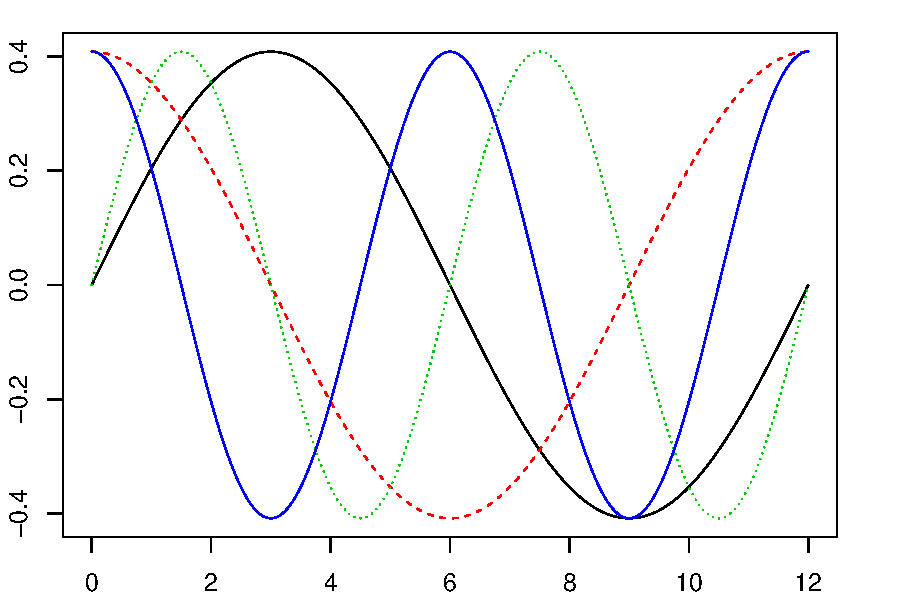
\includegraphics[width=0.8\textwidth]{anexos/base_fourier}
  \caption{Exemplo de base Fourier utilizando 5 funções. Função constante não está representada.}
  \label{fig-base-fourier}
\end{figure}

\subsubsection*{Base B-splines} \label{sub:Base-B-splines}

Funções spline constituem uma base indicada para  dados que possuem natureza não-periódica. 
Cada uma das funções $\phi_k$ é um polinômio, de uma ordem $m$ pré-estabelecida. 
Como regra de bolso, escolhe-se o grau do polinômio como duas unidades a mais que o número de vezes que a função será derivada.
A grande diferença entre uma base utilizando splines e uma base polinomial convencional é que cada uma das funções da base spline estará definida apenas para um subintervalo do intervalo $[t_0,t_1]$ no qual  deseja-se aproximar a função $f(t)$.
Os locais em que se dividem o intervalo total são pontos denominados de breakpoints.

A base B-spline é um conjunto específico de funções que são adequadas para fazer a aproximação desejada.
A literatura cita vantagens computacionais em se utilizar uma base B-splines em relação a outras, tanto no tempo de estimação dos coeficientes $\hat{c}_k$ como na disponibilidade de pacotes que o implementam em diversas linguagens e softwares diferentes.
Uma referência para aprofundar mais no estudo de splines pode ser encontrada em \citeonline{de_boor_practical_1978}. Um exemplo de base de B-splines com polinômios de grau 4 e 4 \emph{breakpoints} é mostrado na figura~\ref{fig:base-bspline}.
\begin{figure}[h!] 
  \centering
    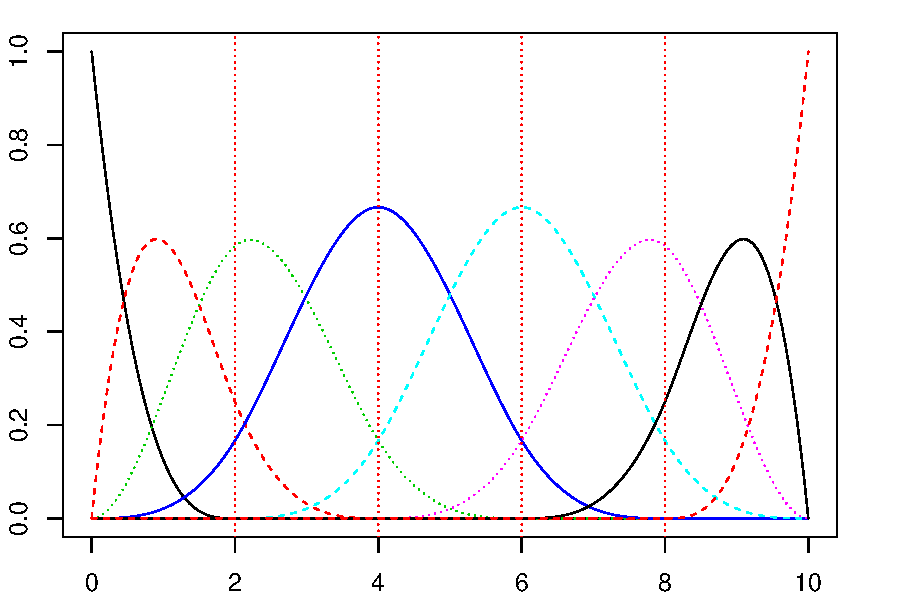
\includegraphics[width=0.8\textwidth]{anexos/base_bsplines1}
  \caption{Exemplo de base B-splines utilizando 10 funções}
  \label{fig:base-bspline}
\end{figure}

\subsection{Análise de Componente Principal Funcional}
\label{FPCA}

A Análise de Componentes Principais (PCA) é um método muito utilizado na análise de dados multivariados com grandes dimensões. Como há muitas variáveis explicativas, a contribuição individual acaba sendo pequena. O método consiste em encontrar componentes que expliquem a maior possível variabilidade dos dados. Os componentes devem ser linearmente independentes e devem ser ordenados em ordem decrescente da contribuição para explicar os dados. Para exposição completa do método, ver \citeonline{jolliffe2005principal}

A Análise de Componentes Principais Funcionais (FPCA) é uma extensão do método multivariado para o caso de dados funcionais. 
A FPCA é utilizada, portanto, para reduzir a dimensão de um dado e exibir suas
características mais marcantes de forma mais compreensível e visual. Sendo
$\mathbb{E}(\int\CHI^{2}(t)dt)<\infty$, pelo teorema de Karhunen–Loève é possível igualar uma função a uma soma infinita de funções ortogonais:
\begin{equation}
\CHI(t)=\sum_{k=1}^{\text{\ensuremath{\infty}}}\left(\int\CHI(t)v_{k}(t)dt\right)v_{k},
\end{equation}
em que $v_{1},v_{2},...,$ são as autofunções ortonormais do operador de covariância
\begin{equation}
\Gamma_{\CHI}(s,t)=\mathbb{E}(\CHI(s)\CHI(t))
\end{equation}
associados aos autovalores $\lambda_{1}\geq\lambda_{2}\geq...$ .
Tomando um um número finito de autofunções, temos uma aproximação da função original, representada através das autofunções e seus coeficientes:
\begin{equation}
\tilde{\CHI}^{(q)}=\sum_{k=1}^{\text{\ensuremath{q}}}\left(\int\CHI(t)v_{k}(t)dt\right)v_{k}.
\end{equation}
Exemplos de utilização da FPCA incluem desde a análise da trajetória de vida de criminosos \cite{ramsay_applied_2002} até o estudo de anormalidades na córnea do olho humano \cite{locantore_robust_1999}

\subsection{Modelo linear funcional}

Enquanto o modelo linear multivariado inclui um número finito de variáveis explicativas, o caso funcional possui infinitos. O modelo linear funcional é definido pela equação abaixo:
\begin{equation}
Y_{i}=\alpha_{i}+\intop_{0}^{T}\rho(t)\chi_{i}(t)dt+\varepsilon_{i},\label{eq:modelofuncionallinear}
\end{equation}
em que $\alpha$ é o intercepto, $\chi(t)$ é a função que representa
cada dado funcional, $\rho(t)$ é o parâmetro único da regressão funcional
paramétrica e $\varepsilon_{i}$ é o termo de erro associado.

A modelagem de dados funcionais, no entanto, requer cuidados adicionais. Fazendo um paralelo ao caso multivariado, há problemas quando
o tamanho da amostra é menor do que o número de variáveis explicativas.
Seja
\begin{equation}
Y=X\beta+\varepsilon
\end{equation}
o modelo a ser estimado, se $X$ for uma matriz com o número de colunas
maior que o de linhas, necessariamente haverá variáveis livres. Assim,
diferentes valores de $\beta$ podem ser utilizados para gerar os
mesmos valores de $Y$. Além disso, é muito provável que o espaço
gerado pela matriz $X$ possua uma dimensão maior que a dimensão de
Y, tornando possível encontrar soluções em que $\varepsilon_{i}=0$,
para todo $i$. 

Uma modelagem em que o modelo se ajusta perfeitamente aos dados (denominado
\emph{overfitting}) não é interessante, pois sua variabilidade será
muito alta. Modelos com alta variabilidade possuem capacidade preditiva
pobre, sendo péssimos em generalizar os dados e dando muita ênfase
ao ruído presente. 

Como um dado funcional está avaliado num espaço infinito dimensional,
o modelo apresentado na equação (\ref{eq:modelofuncionallinear})
também possuirá excesso de variáveis explicativas em relação à amostra.
Dessa forma, alguma estratégia deve ser montada para realizar a regularização,
isto é, impedir o \emph{overfitting} de ocorrer. A seguir, duas maneiras
de realizar a regularização serão apresentadas: a primeira delas é
restringir a quantidade de funções base para tirar a capacidade de
ajuste perfeito aos dados, e a segunda é atribuir uma penalização
para as flutuações da função modelada.


\subsubsection*{Regularização usando funções base restritas}

Sejam $\theta_{0},\theta_{1},...$ e $\psi_{0},\psi_{1},...$ bases
funcionais escolhidas, %(\ref{sub:Bases-para-representa}),
e seja $K_{\beta}$ a quantidade de funções base utilizadas em
\begin{equation}
\beta(t)=\sum_{k}^{K_{\beta}}b_{k}\theta_{k}(t)\quad ou\quad\beta=\boldsymbol{\theta'b}
\end{equation}
tal que a perda de informação ao modelar $\beta$ não seja grande
ao se modelar a variável explicativa. Ao mesmo tempo, toma-se $K_{z}$
da mesma forma para que
\begin{equation}
\chi_{i}(t)=\sum_{k}^{K_{z}}c_{ik}\psi_{k}(t)\quad ou\quad\chi(s)=\boldsymbol{C\psi(t)}
\end{equation}
também não tenha grande perda de informação nem \emph{overfitting}.
$C$ é uma matriz $N \times K_{z}$, em que $N$ representa o tamanho da amostra. Assim, o
modelo (\ref{eq:modelofuncionallinear}) pode ser reescrito da seguinte
forma:
\begin{equation}
\hat{Y_{i}}=\intop_{0}^{T}\rho(t)\chi(t)dt=\intop_{0}^{T}\boldsymbol{C}\psi(t)\theta(t)'\boldsymbol{b}\, dt=\boldsymbol{C}\boldsymbol{J}_{\psi\theta}\boldsymbol{b},
\end{equation}
em que $\boldsymbol{J}_{\psi\theta}$ é uma matriz $K_{z} \times K_{\beta}$
definida por:
\begin{equation}
\boldsymbol{J}_{\psi\theta}=\int\psi(t)\boldsymbol{\theta}'(t)\, dt.
\end{equation}

\subsubsection*{Regularização com penalização por não-suavidade}

Considere o seguinte problema de minimização dos resíduos quadráticos
penalizado:
\begin{equation}
PENSSE_{\lambda}(\alpha,\beta)=\underbrace{\sum_{i=1}^{N}[y_{i}-\alpha-\int z_{i}(t)\beta(t)dt]^{2}}_{g}+\lambda\underbrace{\int[L\beta(t)]^{2}dt}_{h},\label{eq:pensse}
\end{equation}
em que $L$ é um operador diferencial linear adequado para o problema.
Enquanto $g$ penaliza a distância ao quadrado entre a variável resposta
e a variável real, o $h$ penaliza a falta de suavidade do modelo.
Assim, o parâmetro $\lambda$ irá ponderar o grau de suavização da
curva. Caso se tome $\lambda=0$, a curva vai se ajustará perfeitamente
aos dados, e se estará diante de um problema de \emph{overfitting}. Por outro lado,
quando $\lambda\rightarrow\infty$, a regressão será uma curva completamente
suave.

Há duas maneiras de escolher o valor de $\lambda$. A primeira é fazê-lo
de forma subjetiva, isto é, fazendo variar o parâmetro e escolher
a que mais agrade visualmente. A segunda é escolher automaticamente
através de um procedimento de \emph{cross-validation} \footnote{\emph{Cross-validation} é uma forma de determinar um parâmetro com base em previsões dentro da própria amostra.} 
realizado da seguinte forma:
\begin{enumerate}
\item Obtém-se as estimativas de $\alpha_{\lambda}^{(-i)}$ e $\beta_{\lambda}^{(-i)}$,
obtidas encontrando os valores de $\alpha$ e $\beta$ que minimizam
a equação (\ref{eq:pensse}) de toda a amostra, com exceção dos valores
em $(z_{i},y_{i})$. Esta maneira de retirar apenas um valor para previsão é chamada de \emph{leave-one-out}.
\item Monta-se a função 
\[
CV(\lambda)=\sum_{i=1}^{N}[y_{i}-\alpha_{\lambda}^{(-i)}-\int z_{i}(t)\beta_{\lambda}^{(-i)}(t)dt]^{2}.
\]
Escolhendo $\lambda$ de forma a minimizar a função $CV(\lambda)$
será a escolha ótima do parâmetro utilizando esse procedimento de
\emph{cross-validation}.
\end{enumerate}

\subsection{Séries temporais funcionais}

É possível fazer a modelagem de uma série temporal funcional pela decomposição da série em fatores utilizando FPCA. Seja a série temporal $\{ \chi_t(\tau) \}_{t=t_1}^{t_2}$ estimada no  intervalo $[t_a,t_b]$. Haverá, portanto, $n=t_b-t_a+1$ funções representando a série temporal:
\begin{equation}
\chi_{t_1}(\tau), \chi_{t1+1}(\tau), \dots, \chi_{t2}(\tau)
\end{equation}
Assim como demonstrado na seção~\ref{FPCA}, cada função pode ser aproximada pela combinação linear das autofunções ortonormais do operador de covariância:
\begin{equation}
\widetilde{\chi}_s(\tau)=\sum_{i=1}^{m}{ \underbrace{ \left(  \int \chi_s(\tau)  v_i(\tau)dt \right) }_{\phi_{i,t}} } v_i,
\end{equation}
em que $m$ é o número de fatores principais.
Tomando $t$ no intervalo $[t_1,t_2]$, tem-se uma série temporal de $\phi_i$ associada a cada autofunção. Essa série, por sua vez, pode ser estimada com algum método de séries temporais univariadas tradicional, como um modelo ARIMA, passeio aleatório, suavização exponencial, etc. A partir da estimação, pode-se prever cada um dos $\hat{\phi}_{i,t_2+h}$, para cada horizonte de interesse $h$. A curva prevista $\chi_{t_2+h}(\tau)$ é obtida quando se somam os produtos das autofunções com seus respectivos coeficientes previstos, isto é:
\begin{equation}
\hat{\chi}_{t_2+h}(\tau)= \sum_{i=1}^{m}{\hat{\phi}_{i,t_2+h} v_i(\tau) }.
\end{equation}

As séries temporais funcionais foram utilizadas na previsão da ETTJ por \citeonline{hays_functional_2012}, com resultados muito bons. Como é uma abordagem funcional já utilizada na literatura, será implementada para comparação com os resultados obtidos pela estimação com métodos de NP-FDA.

\section{Métodos Não-paramétricos para a Análise de dados funcionais}

Nesta seção, será estudada a metodologia não-paramétrica para análise
de dados funcionais. Ao contrário dos modelos paramétricos, desta
vez não será suposta nenhuma forma funcional para a estimação. Assim,
o modelo tomará a seguinte forma:
\[
Y=r(\chi)+erro,
\]
em que $r(\cdot)$ é um operador linear contínuo de um espaco infinito dimensional $\mathcal{H}$
em $\mathbb{R}$. A maioria das funções utilizadas para implementação
podem ser encontradas em \emph{http://www.lsp.ups-tlse.fr/staph/npfda. }

\subsection{Funções Kernel}

Enquanto no caso multivariado normalmente se utiliza funções Kernel simétricas (ver \citeonline{wand_kernel_1995}), para dados funcionais utiliza-se funções Kernel assimétricas, tais que $\int K = 0$, com suporte compacto em $[0,1]$ (à exceção do Kernel gaussiano, que possui suporte em $[0,\infty)$) e tais que $\forall u \in (0,1), K(u) > 0$. O motivo de se utilizar funções Kernel assimétricas é o fato de as semi-métricas utilizadas para medir a distância entre as curvas produzirem apenas valores positivos. As funções Kernel serão utilizadas pelos métodos não-paramétricos estudados a seguir, e possuem como finalidade atribuir peso localmente às variáveis da amostra.

Seja $I_R(u)$ uma função definida como $1$, quando $u \in \mathbb{R}$ e 0, caso contrário, as funções Kernal mais utilizadas são as seguintes:
\begin{description}
	\item[Kernel uniforme] $K(u)= I_{[0,1]}(u)$
    \item[Kernel triangular] $K(u)= 2(1-u)I_{[0,1]}(u)$
    \item[Kernel quadrático] $K(u)= \frac {3}{2} (1 - u^2) I_{[0,1]}(u)$
    \item[Kernel gaussiano] $K(u)= \frac {\sqrt{2}}{\sqrt{\pi}} exp{-\frac{u^2}{2}} I_{[0,\infty]}(u)$
\end{description}

\subsection{Regressão não-paramétrica funcional}
\label{metodos-previsao-npfda}

Seja $(\chi_i,Y_i)_{i=t_i,...,t_f}$ pares de variáveis aleatórias funcionais identicamente distribuídos como $(\CHI,\boldsymbol{Y})$, tomando valor em $E \times \mathbb{R}$, em que $(E,d)$ é um espaço semi-métrico. O objetivo da regressão é encontrar o valor mais provável para a resposta escalar $Y$ dada a variável funcional observada $\chi$.
Utiliza-se um regressor não linear $r(\chi)=E(Y|\boldsymbol{\chi}=\chi)$
e a previsão por esse método será dada por:
\[
\hat{y}=\hat{r}(\chi).
\]
Para a estimação de $\hat{r}(\chi)$, é proposta a utilização do estimador
não paramétrico utilizando-se uma função kernel assimétrica $K$. Considere que os pesos das curvas são dados por
\begin{equation} \label{peso-local}
\Delta_i=\frac{K(h^{-1}d(\chi,\boldsymbol{\chi}_{i})}{\mathbb{E} \left( K(h^{-1}d(\chi,\CHI_{i}) \right)}.
\end{equation}
A regressão não-paramétrica funcional será uma extensão do estimador de Nadaraya-Watson (empregado comumente para dados em espaço com número finito de dimensões) para o caso funcional. 
Assim, quando se atribui pesos localmente utilizando dados funcionais, sua média ponderada resultará no estimador da regressão funcional
\begin{equation} \label{eq:regressao-npfda}
	\hat{r}(\chi) = \sum_{i=1}^n \Delta_i Y_i.
\end{equation}

Outra variável importante, tratada mais adiante, é a escolha da \bw. Como é a \bw~quem determina o peso de cada curva na estimação, ela possui grande influência nos resultados das previsões pelo método Kernel.

\citeonline{ferraty_nonparametric_2007} investigam aspectos teóricos sobre a regressão com NP-FDA, mostrando uma aplicação do método aplicado a um problema de quimiometria. Já \citeonline{barrientos-marin_locally_2010} implementam a generalização do estimador \emph{local linear} para o caso funcional.



\subsection{Medindo a distância entre as curvas utilizando seminormas} \label{sub:semimetricas}

Nas seções anteriores, utilizou-se a função $d(\cdot,\cdot)$ para expressar
a distância entre duas curvas. Medir a distância entre variáveis é
simples quando trabalhamos no espaço $\mathbb{R}^{p}$, sendo $p$
um número finito. Isso ocorre pois há equivalência entre todas as
normas em espaços de dimensões finitas. Podendo-se utilizar, por exemplo,
a norma euclidiana $||\cdot||$%
\footnote{Seja $x=(x_{1},...,x_{p})^{T}$ um vetor pertencente a $\mathbb{R}^{p}$,
então$||x||^{2}=\sum_{j=1}^{p}(x_{j})^{2}=x^{T}x$.%
} . A escolha da norma num modelo multivariado não será uma tarefa
que requer atenção.

Por outro lado, as variáveis funcionais tomam valores num espaço infinito
dimensional. Em espaços dessa dimensionalidade, a equivalência de normas não se
aplica. Além disso, a utilização de uma métrica pode não ser interessante
por ser muito restritiva. Por isso, $d(\cdot,\cdot)$ será escolhida como
uma semi-norma, dentro de um espaço semi-métrico, ao invés de uma
norma num espaço métrico. As duas gozam das mesmas propriedades, com
exceção de que para a semi-norma vale que $d(x,y)=0\nRightarrow x=y$. 

A escolha da semimétrica utilizada tem papel fundamental no resultado das estimações, pois mudando a forma como se define as distâncias entre as curvas muda-se também as respostas escalares que serão levadas em conta. Assim, a seguir apresenta-se, a seguir, duas famílias de semimétricas

\subsubsection{Semimétrica baseada em Análise de Componente Principal Funcional
(FPCA)}

A FPCA é utilizada para reduzir a dimensão de um dado e exibir suas
características mais marcantes de forma mais compreensível. Sendo
$\mathbb{E}(\int\CHI^{2}(t)dt)<\infty$, podemos reescrever $\CHI$
como a sua expansão pela combinação linear de seus componentes principais:
\begin{equation}
\CHI=\sum_{k=1}^{\text{\ensuremath{\infty}}}\left(\int\CHI(t)v_{k}(t)dt\right)v_{k},
\end{equation}
em que $v_{1},v_{2},...,$ são as autofunções ortonormais do operador de covariância
\begin{equation}
\Gamma_{\CHI}(s,t)=\mathbb{E}(\CHI(s)\CHI(t))
\end{equation}
associados aos autovalores $\lambda_{1}\geq\lambda_{2}\geq...$ .
Tomando um um número finito de autofunções, temos:
\begin{equation}
\tilde{\CHI}^{(q)}=\sum_{k=1}^{\text{\ensuremath{q}}}\left(\int\CHI(t)v_{k}(t)dt\right)v_{k}.
\end{equation}
Dessa forma, é construída uma família de semimétricas com parâmetro
$q$:
\begin{equation}
d_{q}^{PCA}(\CHI_{i},\chi)=\sqrt{\sum_{k=1}^{\text{\ensuremath{q}}}\left(\int[\CHI_{i}(t)-\chi(t)]v_{k}(t)dt\right)^{2}}
\end{equation}



\subsubsection{Semimétrica baseada em derivativas}

É possível construir outra família de semimétricas a partir da distância
entre seus derivativos, da forma a seguir:
\begin{equation}
d_{q}^{deriv}(\CHI_{i},\chi)=\int\left(\CHI_{i}^{(q)}(t)-\chi^{(q)}(t)\right)^{2}dt,
\end{equation}
onde $\chi^{(q)}(t)$ representa a $q$-ésima derivada de $\chi(t)$.
Para o cálculo da derivativa, primeiro os dados serão expandidos na
base B-splines, conforme mostrado na seção (\ref{sub:Base-B-splines}).
Após, pode-se derivar a função Spline na ordem desejada para calcular
a distância entre $\chi$ e $\CHI_{i}$.

É importante enfatizar que, como foi feita a substituição das funções
$\chi$ e $\CHI_{i}$ por funções Spline $S_{1}(t)$ e $S_{2}(t)$
que as representam, é possível trabalhar com dados desbalanceados,
isto é, cujas observações não foram feitas nos exatos mesmos pontos
de $t$. No entanto, salienta-se que o método de representação de
uma função $f(t)$ por meio de uma função Spline $S(t)$ funciona
bem quando $f(t)$ é uma função suave.


%-----------------------
% Metodologia
%-----------------------

\chapter{Metodologia} \label{ch:metodologia}

Para a realização das estimações da ETTJ, os métodos utilizados serão aqueles apresentados na revisão de literatura, tanto para o caso paramétrico quanto para o não-paramétrico. Assim, o estudo será relativamente abrangente em relação à adequação da abordagem funcional para a modelagem do problema em questão.

Como estratégia de avaliação, a amostra será dividida em 2 partes. Os métodos de estimação serão aplicados à primeira parte da amostra, e a previsão é feita dessa primeira parte da amostra. A segunda parte utilizada como verificação da capacidade de previsão. Assim, pode-se calcular o erro das previsões com alguma métrica escolhida e comparar suas performances. 

\section{Dados}

Os dados utilizados serão dados mensais no período de 30/01/1970 até 31/12/2009, constituindo 480 observações da taxa de juros para títulos de maturidades diversas (3, 6, 9, 12, 15, 18, 21, 24, 30, 36, 48, 60, 72, 84, 96, 108 e 120 meses). A figura~\ref{fig:est-termo} contém as séries temporais das diferentes maturidades. 
A base de dados foi construída a partir das taxas \emph{forward} não suavizadas de \citeonline{fama1987information}, disponíveis nos arquivos do CRSP (\emph{Center for Research in Security Prices}). A transformação em Taxas de Juros foi feita por \citeonline{Jungbacker_2013}, e está disponível publicamente no arquivo de dados do \emph{Journal of Applied Econometrics}, como parte do material suplementar.

\begin{figure}[h!] 
  \centering
    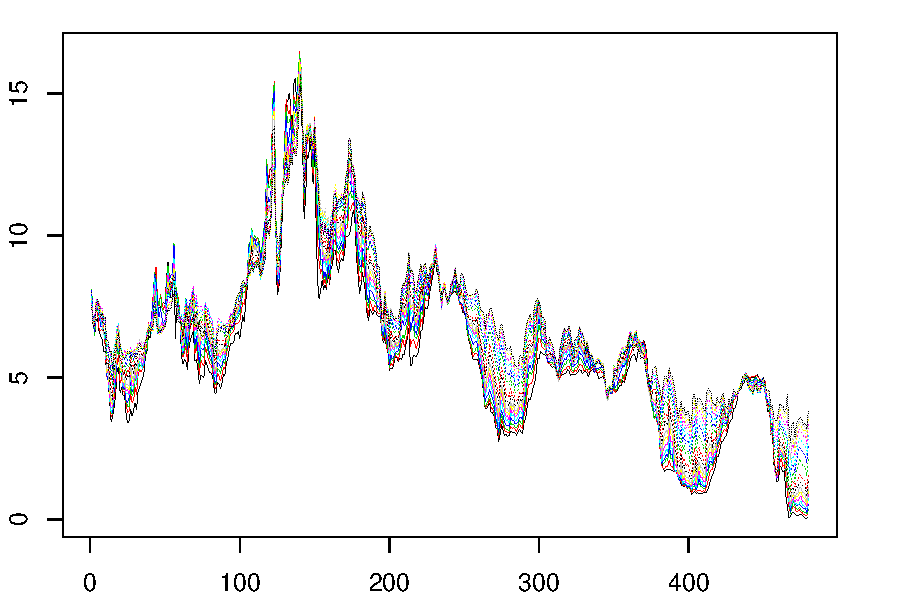
\includegraphics[width=0.8\textwidth]{anexos/taxas_juro}
  \caption{Estrutura a termo da taxa de juros}
  \label{fig:est-termo}
\end{figure}

Como se está interessado na previsão dos valores da taxa de juros fora da amostra, este trabalho modela cada dado funcional como uma observação no tempo $t$ de $\chi_t(\tau)$. A função $f_t:[\tau_1,\tau_k] \rightarrow \mathbb{R}$ é construída com base nos valores discretos ${\tau_1, ..., \tau_k}$, em que $k$ é o número total de maturidades. 

\section{Implementação}

A implementação é feita em R, uma linguagem de programação construída dentro da lógica de software livre. Ela é usada predominantemente para solucionar problemas estatísticos. Por ser livre, é amplamente incrementada por pesquisadores, possuindo um enorme banco de funções e pacotes. O ambiente de programação que será utilizado é o \emph{software} RStudio.

Para cada valor previsto, estima-se o modelo em uma dada janela num intervalo $[t_a,t_b]$, e prevê-se o valor de  $\hat{y}_{t+h|t}(\tau_i)$, em que $h$ é o horizonte da previsão e $\tau_i$ o valor da maturidade. Assim, para cada valor previsto, utiliza-se uma janela que termina $h$ unidades de tempo anteriores à previsão.

Dois tipos de janela móvel são utilizados: com \textbf{tamanho fixo} e \textbf{tamanho expansível}. 
No primeiro tipo, a janela de estimação possui tamanho fixo. Então, enquanto utiliza-se a janela $[t_a,t_b]$ para estimar o modelo e fazer a previsão do valor de $\hat{y}_{t+h|t}(\tau_i)$, a janela $[t_{a+1},t_{b+1}]$ é utilizada para prever o valor de $\hat{y}_{t+1+h|t+1}(\tau_i)$. Quando trabalha-se com tamanho expansível, o ponto de início do intervalo se mantém, mas o final dele é incrementado: utilizam-se os intervalos $[t_{a},t_{b}] ,[t_{a},t_{b+1}],[t_{a},t_{b+2}],\dots$  pra prever $\hat{y}_{t+h|t}(\tau_i),\hat{y}_{t+1+h|t}(\tau_i),\hat{y}_{t+2+h|t}(\tau_i),\dots$, respectivamente. O tamanho da janela começa com 120 observações. Este número se mantém estável quando trabalha-se com tamanho fixo, e aumenta em uma unidade para cada novo unidade que avança no tempo quando se utiliza tamanho expansível.

Quando o tamanho expansível é utilizado, obtém-se o aproveitamento máximo dos dados disponíveis para efetuar a previsão, já que todo valor conhecido pode ser utilizado, enquanto quando trabalha-se com janela fixa, a parte inicial da amostra vai sendo descartada à medida que a janela avança. Ter mais dados é essencialmente importante quando se utiliza métodos cuja convergência dos parâmetros aos seus valores verdadeiros é mais lenta, como ocorre normalmente com os métodos não-paramétricos. 

Os horizontes de previsão trabalhados são: 1 mês, 3 meses, 6 meses e 1 ano.
A primeira janela de estimação compreende 120 observações (um período de 10 anos), entre jan/1984 e dez/1993, para prever os valores entre jan/1994 e dez/1994. A última janela é entre jan/1999 e nov/2008 para tamanho fixo e entre jan/1984 e nov/2008 para tamanho expansível. Ambas preveem, no último período, os valores da taxa de juros entre jan/2009 e dez/2009.

\section{Previsão com Métodos não-paramétricos para Análise de Dados Funcionais} \label{metodologia-npfda}

O objetivo do problema é prever a resposta escalar de um preditor funcional $\chi$ utilizando o método apresentado na seção \ref{metodos-previsao-npfda}. Como a resposta escalar é uma variável unidimensional, e deseja-se fazer a previsão para diversas maturidades, é necessário fazer a estimação para cada uma das maturidades que se deseja realizar previsões.

Como entrada do problema, há $m$ séries temporais de tamanho $n$, em que $m$ é o número de maturidades e $n$ o tamanho do período de tempo no qual as taxas de juro foram observadas. Outra forma de se enxergar a base de dados é através de uma matriz $Y_{m \times n}$, conforme mostra-se a seguir:
\begin{equation} \label{eq:matriz-y}
Y = 
 \begin{bmatrix}
	  y_1(\tau_1) & y_1(\tau_2) & \cdots & y_1(\tau_m) \\
	  y_2(\tau_1) & y_2(\tau_2) & \cdots & y_2(\tau_m) \\
	  \vdots  & \vdots  & \ddots & \vdots  \\
	  y_n(\tau_1) & y_n(\tau_2) & \cdots & y_n(\tau_m)
 \end{bmatrix}_{n \times m}
\end{equation}
Assim, sendo $[t_a,t_b]$ o intervalo para estimação e $h$ o horizonte para previsão desejado, cada dado funcional $\chi_t(\tau)$ pertencente à amostra é formada pela sequência dos valores discretos das linhas de $Y$: $\left( y_1(\tau_1), y_1(\tau_2), ..., y_1(\tau_m) \right)$. 
A resposta escalar associada a esta curva de índice $t$ é $y_{t + h}(\tau_i)$, levando em conta que se está fazendo previsão para o horizonte $h$ e maturidade $\tau_i$. A amostra inicial é composta dos pares $(\chi_j,y_{j+h}(\tau_i)_{j=t_a,...,t_b-h}$. Para a previsão do valor de $y_{t_b+h}(\tau_i)$, por exemplo, toma-se $E(Y|\CHI=\chi_t)$. Para o caso específico do exercício de previsão, o estimador apresentado na equação~\ref{eq:regressao-npfda} ficaria:

\begin{equation}
y_{t+h}(\tau_i)=\hat{r}(\chi_t) = 
\frac
	{\sum \limits_{j=t_a}^{t_b-h} K(d_{q}(\chi_t,\chi_j)/h)y_{j+h}(\tau_i)}
	{\sum \limits_{j=t_a}^{t_b-h}K(d_{q}(\chi_t,\chi_j)/h)}.
\end{equation}


Uma análise preliminar mostrou que, caso a estimação fosse feita sem nenhum tratamento aos dados, os resultados seriam insatisfatórios. Isto ocorre pois o nível da curva é um dos fatores mais significativos para prever os valores futuros da taxa de juros (uma das razões pelas quais, embora muito simples, o passeio aleatório ainda é um método tido como \emph{benchmark} em trabalhos de previsão de curvas de juros). Assim, a matriz $D$ formada pelas distâncias entre curvas $d(\chi_i,\chi_j)$ possuirá valores mais altos, no geral. Como o fator mais decisivo para a proximidade passa a ser o nível das curvas, perde-se a maior vantagem em utilizar métodos funcionais, que é justamente levar em consideração o formato da função.

Por essa razão, decidiu-se retirar o nível da curva para testar o método. Isto, porém, levanta outra questão: qual é o valor que representa o nível da curva? A média, alguma maturidade, ou ainda outro valor? Levando isso em conta, considera-se um modelo mais geral de estimação, apresentado a seguir:
\begin{equation}
\hat{y}_{t+h}(\tau_i) - k_t = \hat{r}(\chi - k_t),
\end{equation}
em que $k \in \mathbb{R}$. Caso $k=0$, tem-se o modelo padrão
\begin{equation}
\hat{y}_{t+h}(\tau_i) = \hat{r}(\chi),
\end{equation}
e quando $k_t = \hat{y}_{t+h}(\tau_i)$, tem-se o modelo de estimação em diferença
\begin{equation}
\Delta \hat{y}_{t+h}(\tau_i)= \hat{r}(\chi - \hat{y}_{t+h}(\tau_i)).
\end{equation}
Além desses, achou-se interessante atribuir valores mais diversos para $k_t$, de certas maturidades específicas. Assim, também foram utilizados uma maturidade curta ($\tau = 3$ meses), uma média ($\tau = 2$ anos), uma longa ($\tau = 10$ anos) e, por fim, tomar $k_t = \hat{\beta}_{1,t}$, em que $\hat{\beta}_{1,t}$ representa a estimação do primeiro fator no modelo de DL. 

\begin{figure}[htp]
  \centering
  \begin{minipage}[t]{0.45\linewidth}
    \centering
    \begin{minipage}[t]{\linewidth}
      \centering     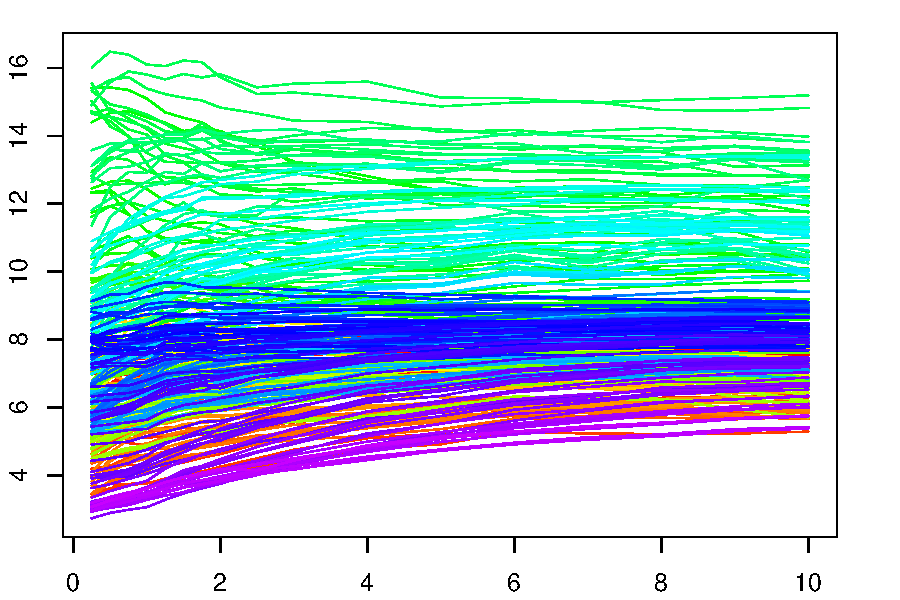
\includegraphics[width=\textwidth]{anexos/perfil_curvas_retira0.pdf}
     \subcaption{$k_t=0$}
    \end{minipage}
    \begin{minipage}[b]{\linewidth}
      \centering     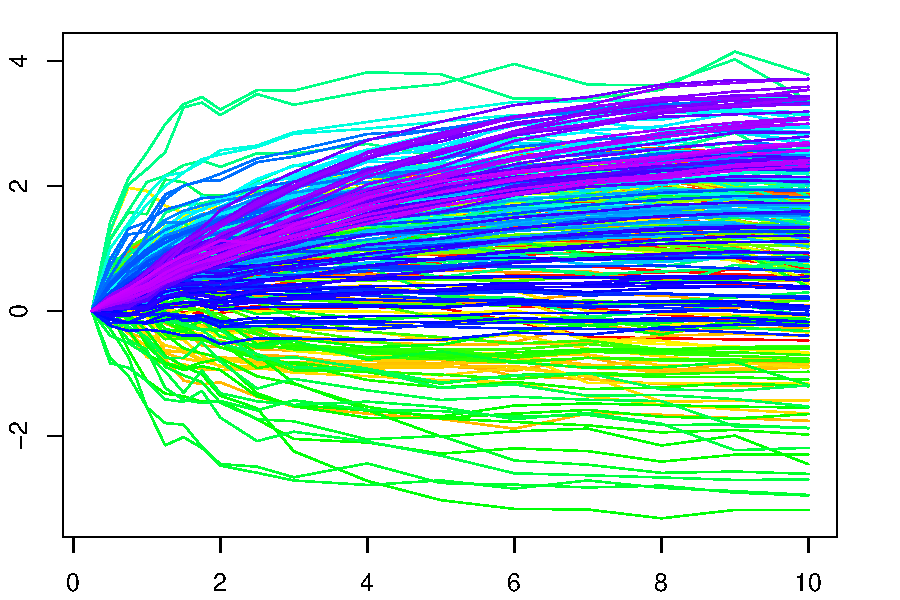
\includegraphics[width=\textwidth]{anexos/perfil_curvas_retira1.pdf} \subcaption{$k_t=y_t(0,25)$}
    \end{minipage}
  \end{minipage}
  \begin{minipage}[t]{0.45\linewidth}
    \centering
    \begin{minipage}[t]{\linewidth}
      \centering     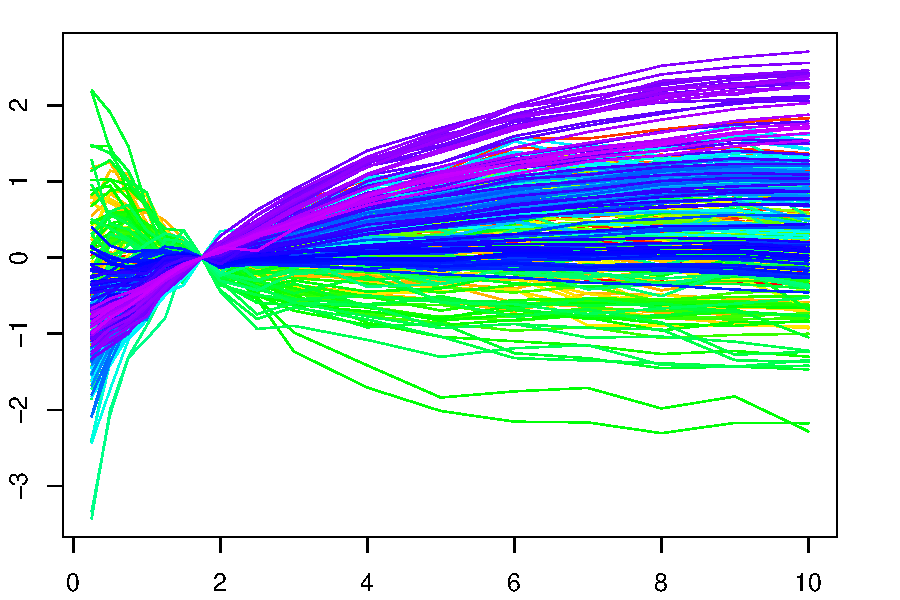
\includegraphics[width=\textwidth]{anexos/perfil_curvas_retira7.pdf}
	\subcaption{$k_t=y_t(2)$}
    \end{minipage}
    \begin{minipage}[b]{\linewidth}
      \centering     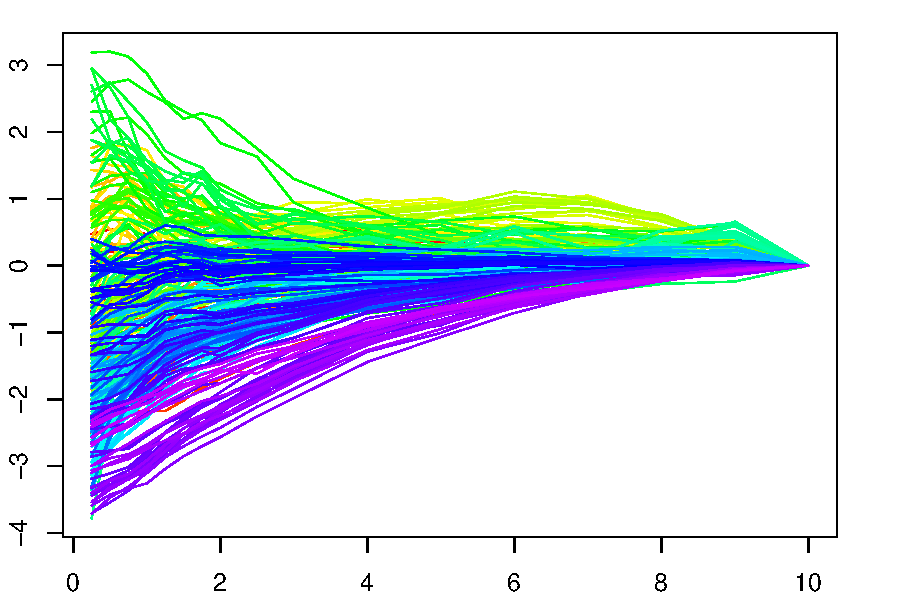
\includegraphics[width=\textwidth]{anexos/perfil_curvas_retira17.pdf} \subcaption{$k_t=y_t(10)$}
    \end{minipage}
  \end{minipage}
  \caption{Curvas $\chi_t(\tau) - k_t$, para valores distintos de $k_t$ e argumento de $y_t$ em anos}
  \label{figuras-retirar-kt}
\end{figure}


\subsection{Escolha da \emph{bandwidth}} \label{sub:bandwidth}

A escolha do valor da \bw~é um fator central na estatística não-paramétrica, já que atua é o elemento principal que atua na suavização da função estimada, possuindo um papel de maior impacto que o da função Kernel. É uma escolha delicada, pois se a variância do modelo for muito alta, o poder de previsão será ruim. No outro extremo, se a suavização for máxima, o modelo estimado será um modelo linear, perdendo características importantes dos dados.

Há duas formas de definir a \bw: utilizando um valor fixo de $h$, ou definindo uma quantidade fixa de curvas para se levar em conta. A seguir, essas duas formas serão apresentadas.

\begin{description}

\item[Utilização de \bw \,fixa:]

Trabalha-se com um valor único para $h$, independente da curva $\chi$ que deseja-se estimar na regressão. Seja a estimação da seguinte forma:

\begin{equation}
R_{CV}^{kernel}(\chi_t) = 
\frac
	{\sum \limits_{j=t_a}^{t_b-h} \left( y_{j+h}(\tau_i)~ K(d_{q}(\chi_t,\chi_j)/h_{opt}) \right) }
	{\sum \limits_{j=t_a}^{t_b-h} K(d_{q}(\chi_t,\chi_j)/h_{opt}) }.
\end{equation}


o valor ótimo para $h_{opt}$ será obtido com base num processo de \emph{cross-validation}. Serão testados valores para $h$ dentro do intervalo $[p(5\%),p(50\%)]$, em que $p(\cdot)$ representa o percentil indicado das distâncias entre pares de curvas $d_q(\cdot,\cdot)$. Assim, o objetivo é encontrar um valor ótimo de $h$:
\[h_{opt} = \operatorname*{arg\,min}_h CV(h),\]
sendo a função $CV(\cdot)$ definida por
\[
CV(h) = \sum \limits_{j=t_a}^{t_b} \left(  y_{j+h}(\tau_i) - R_{(-j)}^{kernel}(\boldsymbol{x}_i)  \right)^2, 
\]
em que
\[
R_{CV}^{kernel}(\chi_t) = 
\frac
	{\sum \limits_{k=t_a, k \neq j}^{t_b-h} \left( y_{k+h}(\tau_i)~ K(d_{q}(\chi_t,\chi_k)/h_{opt}) \right) }
	{\sum \limits_{k=t_a, k \neq j}^{t_b-h} \left( K(d_{q}(\chi_t,\chi_k)/h_{opt}) \right)  }.
\]



\item[Vizinhos mais próximos:]

Aqui, a ideia é testar qual o número de vizinhos mais próximos (isto é, as curvas $j$ com valores de $d(\chi_t,\chi_j)$) a se levar em conta para definir a \bw~que geram as melhores previsões feitas dentro da amostra.
O número de vizinhos se mantém fixo, enquanto o tamanho da \bw~$h_{k_{opt}}(\chi_t)$ varia localmente para manter estável em exatamente $k$ a quantidade de curvas tais que $d_{q}(\chi_t,\chi_{j})/h_{k_{opt}} \in [0,1]$, isto é, estejam dentro do intervalo de suporte da função Kernel assimétrico.

Testa-se os valores de $k$ dentro do intervalo $[10,\dfrac{n}{2}]$, em que $n$ representa o tamanho da janela de estimação. Dentre esses valores, testados, escolhe-se o valor ótimo de vizinhos mais próximos através da minimização da função $GCV(\cdot)$:
\[k_{opt} = \operatorname*{arg\,min}_h GCV(k),\]
em que $GCV(\cdot)$ é definida por
\[
GCV(k) = \sum \limits_{j=t_a}^{t_b} \left(  y_{j+h}(\tau_i) - R_{(-j)}^{kNN}(\chi_j)  \right)^2, 
\]
em que
\[
R_{(-j)}^{kNN}(\chi_j) = 
\frac
	{\sum \limits_{k=t_a, k \neq j}^{t_b-h} \left( y_{k+h}(\tau_i)~ K(d_{q}(\chi_t,\chi_k)/h_{opt}) \right) }
	{\sum \limits_{k=t_a, k \neq j}^{t_b-h} \left( K(d_{q}(\chi_t,\chi_k)/h_{opt}) \right)  }.
\]


Após encontrado o valor de $h_{k_{opt}}$, chega-se no estimador desejado:
\[
R_{GCV}^{kNN}(\chi_t)=
\frac
	{\sum \limits_{j=t_a}^{t_b-h} \left( y_{j+h}(\tau_i)~ K(d_{q}(\chi_t,\chi_j)/h_{k_{opt}}(\chi_t)) \right) }
	{\sum \limits_{j=t_a}^{t_b-h} K(d_{q}(\chi_t,\chi_j)/h_{k_{opt}}(\chi_t) }.
\]


\end{description}

Neste trabalho, limita-se à escolha da \bw~baseada na capacidade de ajuste dentro da amostra, e não na previsão. Espera-se, num trabalho futuro, incorporar também a capacidade preditiva quando feita a \emph{cross-validation}. 

\subsection{Escolha da semimétrica}

As semimétricas serão testadas dentro das duas famílias apresentadas na seção~\ref{sub:semimetricas}: derivadas e FPCA. Em cada uma, é preciso definir um parâmetro: para a primeira, a ordem da derivada, e para a segunda, a quantidade de componentes principais levados em conta.

Uma análise preliminar mostrou que os resultados de previsão eram muito insatisfatórios para derivadas de grau $2$ ou maior. Portanto, usou-se apenas a derivadas de ordem $1$ e a curva sem tomar derivada ($q=0$).

Já para a semimétrica baseada na FPCA, o testes foram feitos para o número de componentes principais $q \in \{1, 2, ..., 9\}$. Destes, a mudança na distância entre as curvas torna-se totalmente irrelevante à medida que o número de componentes é maior do que $5$, e o resultado da previsão muda muito pouco entre tomar $2,3,4$ ou $5$ componentes principais. Além disso, notou-se que quando se toma apenas $1$ componente principal, o resultado da previsão é ruim. Assim, escolheu-se somente utilizar $q=5$.



\section{Previsão com os Métodos escolhidos como \emph{benchmark}}

Para melhor avaliar os resultados dos métodos investigados neste trabalho, compara-se a capadidade de previsão deles com outros métodos utilizados na literatura. São eles: o modelo de DL, o passeio aleatório e o modelo AR(1).

\subsection{Previsão com Método de Diebold-Li}

Seja o modelo de \citeonline{diebold_forecasting_2006} a seguir:

$$y_{t}(\tau)=\beta_{1,t}+\beta_{2,t}\left( \frac { 1-e^{ -\lambda \tau  } }{ \lambda\tau}  \right) -\beta_{3,t}\left( \frac { 1-e^{ -\lambda \tau  } }{ \lambda \tau  } -e^{ -\lambda \tau  } \right),$$
o primeiro passo para realizar as previsões é definir o valor de $\lambda$, que é mantido fixo durante a estimação, ao contrário de quando se utiliza o modelo de NS. 

Para escolher o valor de $\lambda$ emprega-se um método de \emph{cross-validation}. A busca foi realizada tomando valores dentro do intervalo $[0.2,1.2]$, com incrementos de $0.05$. O intervalo de aprendizado foi dividido em duas partes: uma para estimar (contendo 60\% do intervalo) e outra para prever fora da amostra (contendo o resto). Assim, para cada um dos valores testados, as previsões foram feitas e o Erro Quadrático Médio calculado. 
De acordo com as simulações executadas nesse trabalho, tomar $\lambda=0.5$ gerou as melhores previsões dentro do intervalo de aprendizagem.

Uma vez fixo o valor de $\lambda$, pode-se partir para as estimações por completo. Para cada período de $t$, os valores de $\hat{\beta}_{1,t}$, $\hat{\beta}_{2,t}$ e $\hat{\beta}_{3,t}$ são estimadas em \emph{cross-section}. A partir dos valores de  $\hat{\beta_1}$, $\hat{\beta_2}$ e $\hat{\beta_3}$, pode-se recriar a curva de juros para qualquer conjunto de maturidades, inclusive aquelas que não foram utilizadas estimar os $\beta$'s.

Com base nos valores de $\hat{\beta}$ já estimados, prevê-se os valores futuros de $\hat{\beta}$ através de um modelo AR(1), com $h$ passos à frente. 
$$\hat{\beta} _{ t+h/t } = \hat{c} + \hat{\Gamma}\hat{\beta}_t$$
Após, o valor previsto para cada maturidade é obtido após multiplicar $\beta$ pelos fatores.
$$\hat { y } _{ t+h/t }(\tau)=\hat{\beta} _{ 1,t+h/t }+\hat{\beta} _{ 2,t+h/t }\left( \frac { 1-e^{ -\lambda \tau  } }{ \lambda \tau  }  \right) -\hat{\beta} _{ 3,t+h/t }\left( \frac { 1-e^{ -\lambda \tau  } }{ \lambda \tau  } -e^{ -\lambda \tau  } \right)$$


\subsection{Passeio aleatório}
Considera-se a série temporal um passeio aleatório. Assim, para cada qualquer horizonte, considera-se que o valor futuro da maturidade se manterá o mesmo:

\begin{equation}
\hat{y}_{t+h/t}(\tau_i)=y_t(\tau_i).
\end{equation}


\subsection{AR(1)}
Ajusta-se, à cada maturidade da curvas de juros, um modelo autorregressivo de ordem 1, utilizando mínimos quadráticos ordinários:
$$y_t(\tau_i)=\alpha(\tau_i) + \phi(\tau_i) y_{t-1}(\tau_i)+\varepsilon_{t}(\tau_i).$$
Assim, minimizando os valores quadráticos de $\varepsilon$ obtém-se os estimadores de $\alpha(\tau_i)$ e $\phi(\tau_i)$.
Pode-se, então, fazer a estimação $1$ passo à frente utilizando os valores dos coeficientes estimados na equação do modelo:
\begin{equation}
\hat{y}_{t+1/t}(\tau_i)=\hat{\alpha}(\tau_i) + \hat{\phi}(\tau_i) y_t(\tau_i).
\end{equation}

Para prever mais do que 1 passo à frente, é possível utilizar o valor previsto para prever outro passo à frente:
\begin{equation}
\hat{y}_{t+p/t}(\tau_i)=\hat{\alpha}(\tau_i) + \hat{\phi}(\tau_i) \hat{y}_{t+p-1/t}(\tau_i),
\end{equation}
e assim por diante. Iterativamente, consegue-se então utilizar o método para fazer a previsão $n$ passos à frente.

\subsection{Série temporal funcional}

O número de componentes principais utilizados pela FPCA será estimado entre 1 e 5. Similarmente ao que foi discutido no caso das semimétricas baseadas em FPCA, utilizar um número alto de componentes acaba por não mudar os valores previstos, já que cada novo componente explica cada vez uma porção menor da variabilidade dos dados. Assim, pela análise preliminar, utilizar mais que 5 componentes principais (esclarece-se que o mesmo limite de 5 fatores para a série temporal funcional e as semimétricas baseadas em FPCA é uma mera coincidência) não ocasionou nenhuma mudança nas previsões. \citeonline{hays_functional_2012} utilizam 3 fatores, para a comparação com o modelo de DL ser mais direta, avaliando principalmente a diferenciação entre usar fatores pré-determinados pelo modelo ou estimá-los a partir dos dados através de FPCA.
A dinâmica dos fatores será modelada com ARIMA, passeio aleatório e suavização exponencial.

\section{Metodologia para avaliação da performance das previsões} \label{sub:avaliacao}

Para analisar quão boas são as previsões feitas pelos métodos analisados, utiliza-se diversas métricas distintas. Seja $\{y_{t}(\tau_i)\}_{t=t_0}^T$ a série temporal referente à maturidade $\tau_i$ e $\{\hat{y}_{t}^m(\tau_i)\}_{t=t_0}^T$ os valores previstos para um dado método $m$. A série temporal dos erros de previsão para este método será denominada $\{e_{t}^m(\tau_i)\}_{t=t_0}^T$.

\begin{description}
	\item[Raiz do Erro Quadrático Médio] O erro quadrático médio das previsões é um critério estatístico amplamente utilizado na literatura. Pelo erro ser elevado ao quadrado, esse critério pune com mais severamente os desvios grandes da meta. Ele é obtido pela seguinte expressão: \[ REQM^m(\tau_i) = \sqrt{ \frac{1}{n} \sum _{t = t_0}^T (\hat{y}_{t+h|t}^m(\tau_i) - y_{t+h}(\tau_i))^2 }, \]
	em que $n = T - t_0 + 1$.
	\item[Erro Quadrático Acumulado de Previsão] É uma metodologia que não fornece um simples indicador comparativo de performance, mas sim um gráfico do comportamento da previsão do método avaliado com relação a algum outro método que é utilizado como \emph{benchmark}. A fórmula para implementar o método é a seguinte:
	\[ EQAP_{m}(\tau_i) = \sum_{t=t_0}^T  \left[ \left( \hat{y}_{t+h|t}^{benchmark}(\tau_i) - y_{t+h}(\tau_i) \right)^2 - \left( \hat{y}_{t+h|t}^m(\tau_i) - y_{t+h}(\tau_i) \right)^2 \right]. \]
Assim, o trecho em que o gráfico possui inclinação positiva é onde o método avaliado possui performance superior ao \emph{benchmark}, enquanto quando é negativamente inclinado é o método \emph{benchmark} quem possui a melhor performance.

	\item[Significância da diferença de previsão]

Embora alguns métodos possuam resultados melhores, em termos de erro quadrático médio, do que outros, é importante saber o quão melhor um método é e se o resultado e estatisticamente importante. 
Para isso,utiliza-se neste trabalho dois testes comumente empregados na literatura para comparar previsões: o teste proposto por \citeonline{giacomini2006tests} e o teste proposto por \citeonline{diebold2002comparing}.

O teste de Giacomini-White (GW) produz uma estatística sobre a significância da diferença de performance de dois métodos de previsão, supondo que estes são 
produzidos a partir de uma janela móvel de tamanho fixo. A hipótese nula do teste é que os dois métodos comparados, um dado método $m$ e o método \bm, possuem igual capacidade de previsão:
\begin{equation} \label{eq:hip-nula-gw}
\mathbb{H}_0:E[d_{a,t+h}|\delta_{m,t}]=0,
\end{equation}
em que $\delta_{m,t}$ é um vetor $p \times 1$ de funções teste ou instrumentos, $h$ o horizonte de previsão e $d_{m,t}=(e_{benchmark,t})^2 - (e_{m,t})^2$ é o diferencial da perda. A estatística GW é calculada como:
\begin{equation}
GW_{m,n} = n \left( n^{-1} \sum_{t=t_0}^{T} \delta_{m,t} d_{m,t+h} \right)' \hat{\Omega}_n^{-1}	
\left( n^{-1} \sum_{t=t_0}^{T} \delta_{m,t} d_{m,t+h} \right) \overset{d}{\longrightarrow} \chi_{dim(\delta)}^2,
\end{equation}		
em que $\hat{\Omega}_n$ é um estimador HAC (consistente para heterocedasticidade e autocorrelação) para a variância assintótica de $\delta_{m,t} d_{m,t}$ e $n=T-t_0+1$ é o número de previsões fora da amostra realizadas. Dada a hipótese nula em~\ref{eq:hip-nula-gw}, a estatística de teste $GW_{m,t}$ é assintoticamente distribuída como $\chi^2_p$.

Por supor que a janela móvel possui tamanho fixo, o teste de GW não é utilizado para as estimações realizadas com janela de tamanho expansível, para quem será utiliza-se o teste de Diebold-Mariano (DM). Este teste possui como hipótese nula e alternativa:
\begin{equation} \label{eq:hip-nula-dm}
\begin{split}
\mathbb{H}_0:E[d_{a,t+h}|\delta_{m,t}]=0 \\
\mathbb{H}_1:E[d_{a,t+h}|\delta_{m,t}] \neq 0
\end{split}
\end{equation}
A estatística de teste de DM é:
\begin{equation}
DM_{m,t} = \dfrac{\bar{d}}{ \left( \hat{avar}(\bar{d}) \right)^{1/2}} = 
	\dfrac{\bar{d}}{ \left( \hat{LRV}_{\bar{d}} / T \right)^{1/2}} \overset{a}{\longrightarrow} N(0,1)
\end{equation}
em que 
\[ 
\bar{d} = \dfrac{1}{n} \sum_{t=t_0}^T d_{m,t} 
\]
e $\hat{LRV}_{\bar{d}}$ é um estimador consistente da variância assintótica de $\sqrt{T} \bar{d}$.

Dada a hipótese nula em~\ref{eq:hip-nula-dm}, a estatística de teste $DM_{m,t}$ é assintoticamente distribuída como uma normal-padrão.

\end{description}

%---------------------------------
% Resultados
%---------------------------------
\chapter{Resultados} \label{ch:resultados}

As estimações foram feitas com códigos escritos em R, que foram disponibilizados na internet: \emph{https://github.com/mcruas/dissertacao}. Uma breve  explicação está 
disponível no apêndice~\ref{apend:rotinas} deste trabalho, enquanto a versão mais completa do documento está descrita no \emph{site} indicado acima. 
Estimou-se a ETTJ com os seguintes métodos: \textbf{passeio aleatório} (utilizado como \bm ), modelo \textbf{AR(1)}, modelo de \textbf{DL}, \textbf{regressão não-paramétrica para dados funcionais} de diversas combinações de semimétricas e valores de $k_t$ e \textbf{séries temporais funcionais}, também com diferentes números de componentes principais e valores de $k_t$, além de diferentes formas de modelar a dinâmica dos fatores (foi utilizado para isso o passeio aleatório, suavização exponencial e modelo ARIMA).

A primeira pergunta a ser respondida, quando a série começou a ser analisada, é com relação à sua estacionariedade. Para ser considerada estacionária, na sua forma fraca, a série deve ser gerada por um processo de média e desvio padrão constantes. 
Salienta-se, porém, que trabalhando com variável funcional, é necessário que esta variável que seja estacionária, e não a série univariada de cada maturidade, como seria caso fosse aplicada outra metodologia. Embora seja bem possível que quando estacionarizadas as séries de cada maturidade, obtenha-se séries funcionais também estacionárias, a estacionariedade de uma não necessariamente implica na da outra. 
Em um artigo recente, \citeonline{horvath-2014} descreve como testar a estacionariedade para séries temporais funcionais. Neste trabalho, não foi possível implementar este teste, mas é previsto como um próximo passo importante.
Em muitos casos, lança-se mão da diferenciação sucessiva da série para transformar os dados brutos numa série estacionária. Neste trabalho, conforme indicado na seção~\ref{metodologia-npfda}, utiliza-se a subtração de séries distintas para tentar obter uma série temporal mais bem comportada. 
Para todos os valores de $k_t$ descritos, com exceção de quando é identicamente nulo, a série não teve sua estacionariedade rejeitada pelo teste ADF, para nenhuma maturidade. Embora não seja equivalente à série temporal funcional ser estacionário, como dito anteriormente, nota-se que os resultados melhoram quando há esse tratamento. Decidiu-se realizar o mesmo processo de retirar valores das curvas na estimação das séries temporais funcionais. Os valores de $k_t$ utilizados são os mesmos definidos na seção~\ref{metodologia-npfda}.

Em relação às semimétricas escolhidas para a análise com NP-FDA, percebeu-se que a previsão da curva quando utiliza-se a distância das curvas em nível (semimétrica derivada com $d=0$) é extremamente parecida com a previsão quando utiliza-se a semimétrica baseada em FPCA com $q=5$. Por isso, decidiu-se omitir a versão da derivada com $d=0$ dos resultados finais.

\begin{figure}[htp]
  \centering
  \begin{minipage}[t]{0.45\linewidth}
    \centering
    \begin{minipage}[t]{\linewidth}
      \centering     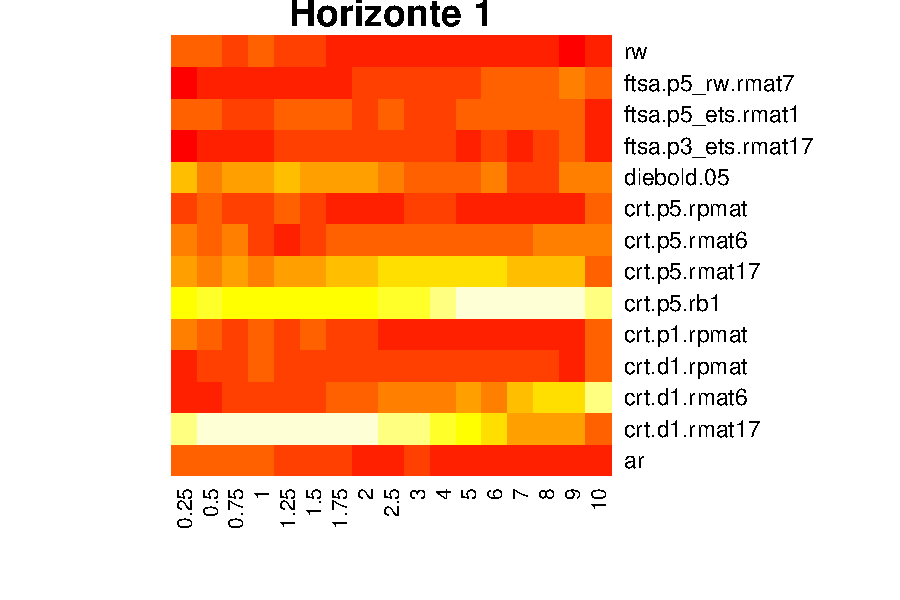
\includegraphics[width=\textwidth]{anexos/heatmap1.pdf}
     
    \end{minipage}
    \begin{minipage}[b]{\linewidth}
      \centering     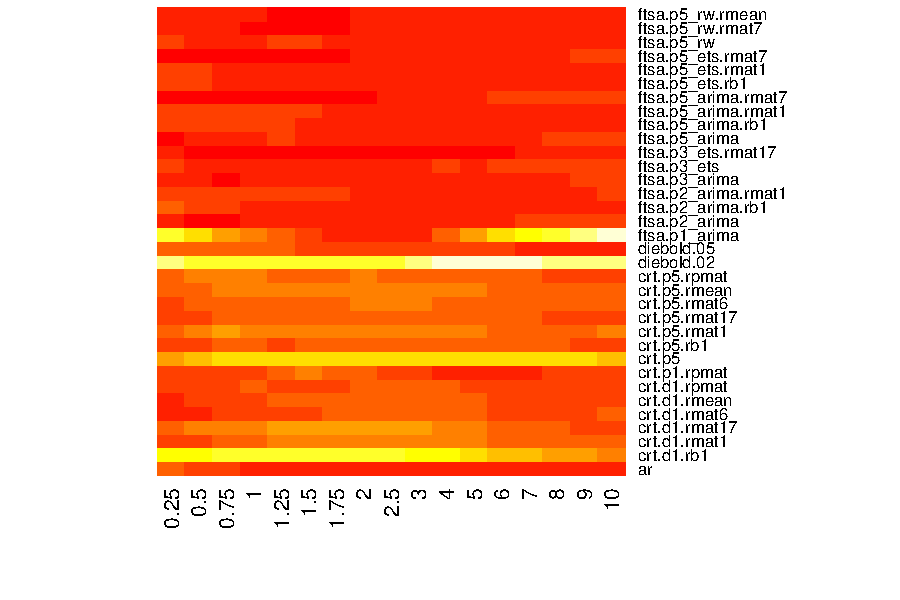
\includegraphics[width=\textwidth]{anexos/heatmap3.pdf} 
    \end{minipage}
  \end{minipage}
  \begin{minipage}[t]{0.45\linewidth}
    \centering
    \begin{minipage}[t]{\linewidth}
      \centering     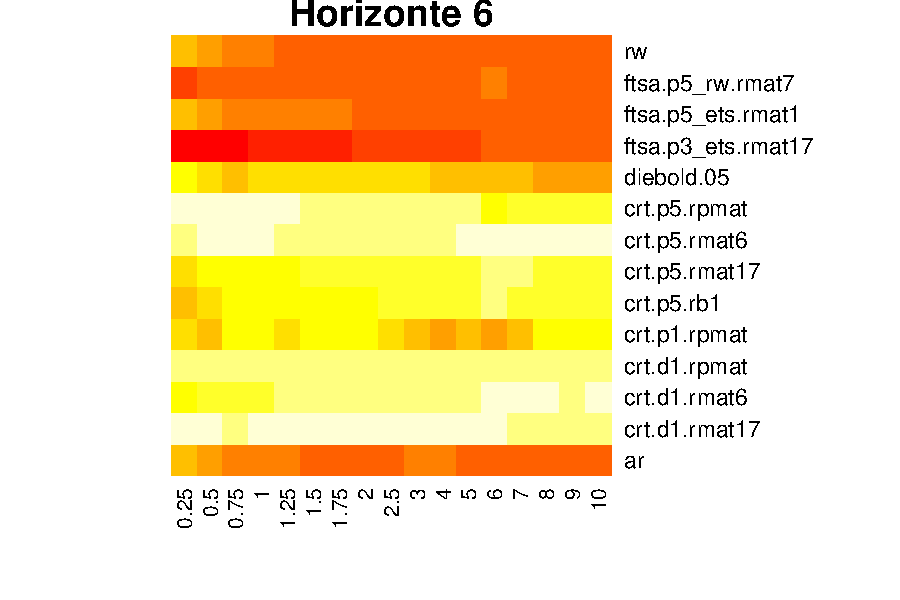
\includegraphics[width=\textwidth]{anexos/heatmap6.pdf}
	
    \end{minipage}
    \begin{minipage}[b]{\linewidth}
      \centering     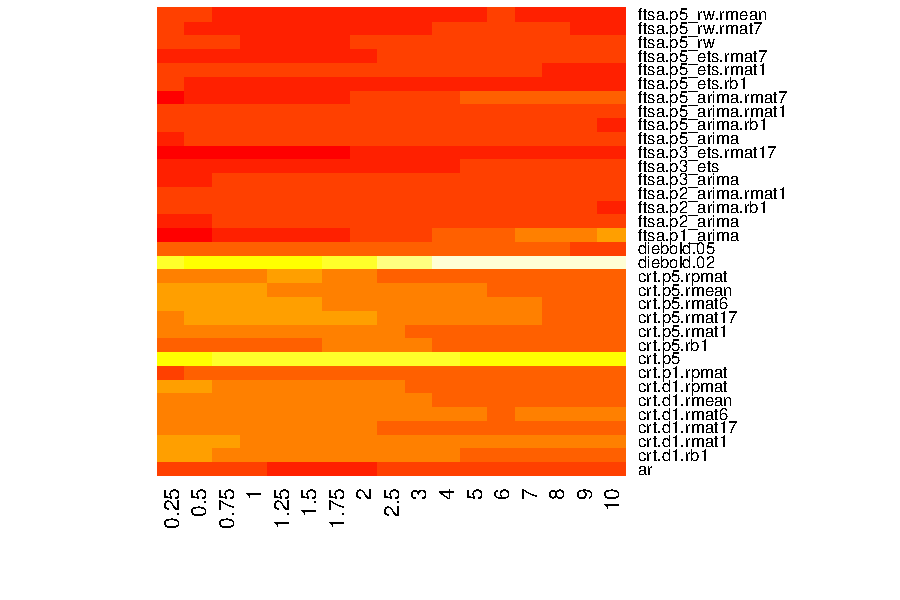
\includegraphics[width=\textwidth]{anexos/heatmap12.pdf} 
    \end{minipage}
  \end{minipage}
  \caption{Gráficos de calor do Erro Quadrático Médio das previsões feitas com janela de tamanho expansível} 
  \label{fig:heatmaps}
\end{figure}

\begin{figure}[h!]
  \centering
  \begin{minipage}[t]{0.45\linewidth}
    \centering
    \begin{minipage}[t]{\linewidth}
      \centering     \includegraphics[width=\textwidth]{anexos/EQAP1-1.pdf}
     
    \end{minipage}
    \begin{minipage}[b]{\linewidth}
      \centering     \includegraphics[width=\textwidth]{anexos/EQAP3-5.pdf} 
    \end{minipage}
  \end{minipage}
  \begin{minipage}[t]{0.45\linewidth}
    \centering
    \begin{minipage}[t]{\linewidth}
      \centering     \includegraphics[width=\textwidth]{anexos/EQAP6-10.pdf}
    \end{minipage}
    \begin{minipage}[b]{\linewidth}
      \centering     \includegraphics[width=\textwidth]{anexos/EQAP12-17.pdf} 
    \end{minipage}
  \end{minipage}
  \caption{Gráficos do Erro Quadrático Acumulado de previsão, para algumas maturidades selecionadas e janela de tamanho expansível} 
  \label{fig:eqap}
\end{figure}


As abreviaturas dos métodos são descritos no apêndice~\ref{apend:legendas}. A diferença entre \texttt{diebold.02} e \texttt{diebold.05} é que o primeiro utiliza $\lambda=0.2$ e o segundo, $\lambda=0.5$. Embora a performance utilizando $\lambda=0.5$ tenha sido, em geral, melhor no estudo com apenas a parte de teste da amostra, decidiu-se manter nos resultados a estimação feita com $\lambda=0.2$ pela performance boa nas maturidades menores.

Os resultados completos das estimações e previsões estão disponíveis no Apêndice~\ref{tabelas-resultados}. Eles estão organizados em tabelas por horizonte (1, 3, 6 e 12 meses) e por tipo de janela (móvel ou expandindo). Nas tabelas comparativas com o passeio aleatório, o valor informado é o Erro Quadrático Médio. A figura~\ref{fig:heatmaps} mostra gráficos de calor para mostrar de forma mais visual o conteúdo de algumas tabelas. Valores de erro maiores são associados à cores mais amareladas, tendendo ao branco quanto piores forem as previsões. Já os métodos que se saíram bem possuem uma cor avermelhada. Já a figura~\ref{fig:eqap} apresenta o Erro Quadrático Acumulado de Previsão, conforme apersentado na seção~\ref{sub:avaliacao}, para alguns horizontes e maturidades.

Analisando os resultados sobre os métodos NP-FDA, foi percebido que quanto maior a maturidade que se faz a previsão, pior foi o desempenho com relação ao passeio aleatório. Igual relação se estabelece quando se aumenta o horizonte de previsão: o desempenho relativo ao passeio aleatório também cai. Um fato importante a se destacar é que, para os métodos NP-FDA, a maioria das variações estimadas obteve melhor desempenho quando utilizada a janela expandida, com relação à janela móvel. O motivo disso é que provavelmente haver mais dados acaba contribuindo significativamente para a melhora do desempenho, possivelmente dada a convergência lenta desses métodos não-paramétricos aplicados a dados funcionais. 
Nas maturidades mais baixas e horizontes menores, é possível achar diversos dos métodos não-paramétricos que são melhores que o passeio aleatório; no entanto, com as maturidades mais altas e horizontes maiores, os métodos aqui propostos não obtêm sucesso.

Enquanto os métodos não-paramétricos apresentam melhora da capacidade preditiva quando a janela com tamanho expansível é empregada, os modelos de DL tiveram piora significativa. Percebe-se, portanto, que ter mais dados pode atrapalhar a estimação da dinâmica dos fatores. É interessante notar que os modelos de DL tiveram melhor desempenho com horizontes mais longos, contrariando a lógica dos outros métodos estimados.

Os métodos \texttt{crt.d1} e \texttt{crt.p5} tiveram desempenho relativamente pior que os outros métodos com NP-FDA, principalmente para horizontes maiores. Isso reforça a importância de se trabalhar com as séries estacionárias, inclusive quando trabalha-se com dados funcionais. 

Com relação aos dois tipos de semimétricas utilizados (primeira derivada e FPCA com 5 componentes principais), não foi percebida melhora significativa de desempenho entre eles. Ora um possui melhores previsões, ora o outro. Sobre os valores $k_t$ utilizados, pode-se perceber uma tendência de melhores resultados quando toma-se $k_t = y_t(\tau_i)$, em que $\tau_i$ é a maturidade a ser prevista. Os métodos que utilizam como $k_t$ o valor da própria maturidade prevista são indicados por \texttt{crt.}\textbf{sm}\texttt{.rpmat}, em que \textbf{sm} indica a semimétrica utilizada.

Os métodos estimados com séries temporais funcionais foram os que tiveram melhor resultado, de modo geral. Em diversos deles, as previsões foram melhor que o passeio aleatório para quase todas as maturidades, e muito superiores ao estimado com os modelos de DL. A dinâmica dos fatores que, aparentemente, deu melhores resultados foi a suavização exponencial. 

% ---
\chapter*[Conclusão]{Considerações Finais} \label{ch:conclusao}
\addcontentsline{toc}{chapter}{Considerações Finais}
% ---

A Estrutura a Termo da Taxa de Juros é objeto de muitos estudos. Mesmo assim, fazer previsões com uma estratégia tão simples como o passeio aleatório permanecer como um \bm~tão utilizado demonstra a dificuldade em se prever essas séries temporais.

O \emph{framework} de dados funcionais é relativamente novo. Como já havia a experiência de bons resultados na previsão da ETTJ utilizando séries temporais funcionais (baseadas em dinâmica de fatores utilizando FPCA) achou-se importante investigar outras variações de métodos que considerassem a natureza funcional do problema. 
Por isso, havia motivação suficiente para testar a capacidade de previsão fora da amostra com métodos não-paramétricos para dados funcionais. 
Os resultados insatisfatórios encontrados, porém, não podem ser encarados conclusivos de que os os métodos com NP-FDA são ruins para o problema, visto que métodos tradicionais também não deram bons resultados na amostra considerada. Como é uma área que no momento de escrita desta dissertação pertence à fronteira do conhecimento, há muita pesquisa sendo feita na base do método que pode melhorar consideravelmente sua performance. 

É possível apontar alguns caminhos interessantes para futuros trabalhos envolvendo dados funcionais e a estimação e previsão da ETTJ, como por exemplo trabalhar com a série diferenciada em relação ao tempo, ao invés de diferenciar com relação à maturidade, como feito aqui. Outra possibilidade é aplicar diretamente o modelo linear funcional para fazer a previsão. Dentro dos próprios métodos NP-FDA, pode-se investigar a utilização do \emph{local linear} ao invés do Nadaraya-Watson. Em um trabalho futuro, também está prevista a inclusão de outra forma de fazer \emph{cross-validation}, incluindo a capacidade de previsão dentro do período de estimação, conforme discutido na seção~\ref{sub:bandwidth}. 



% ----------------------------------------------------------
% ELEMENTOS PÓS-TEXTUAIS
% ----------------------------------------------------------
%\postextual
% ----------------------------------------------------------

% ----------------------------------------------------------
% Referências bibliográficas
% ----------------------------------------------------------
\bibliography{Bibliografia-dissertacao}

% ----------------------------------------------------------
% Glossário
% ----------------------------------------------------------
%
% Consulte o manual da classe abntex2 para orientações sobre o glossário.
%
%\glossary

% ----------------------------------------------------------
% Apêndices
% ----------------------------------------------------------

% ---
% Inicia os apêndices
% ---
\begin{apendicesenv}
%
%% Imprime uma página indicando o início dos apêndices
\partapendices
%

%%%%%%%%%%%%%%%%%% Capítulo Rotinas %%%%%%%%%%%%%%%%%%%%%%%%%%%%
\chapter{Sobre as rotinas utilizadas} \label{apend:rotinas}


Um dos cuidados que se teve na execução deste trabalho foi montar os códigos e rotinas de modo que fosse facilmente reproduzível por quem tivesse interesse. Assim, fica fácil para quem quiser dar continuidade à pesquisa, encontrar melhorias e até potenciais erros no código que influenciem os resultados.

Os códigos estão disponíveis em \emph{https://github.com/mcruas/dissertacao}. Para um início fácil e rápido, recomenda-se clonar o repositório. Instruções para isto estão disponíveis no \emph{site}.

\section{Estimação da ETTJ com NP-FDA}
Para realizar a estimação e previsão da ETTJ, é preciso, primeiro, carregar o arquivo \texttt{biblioteca-npfda-ettj.R}. As funções presentes nesse arquivo foram uma extensão das disponibilizadas em \emph{http://www.math.univ-toulouse.fr/staph/npfda/} como acompanhamento do livro \citeonline{vieu_nonparametric_2006}.

As variáveis necessárias para representar a base de dados são:
\begin{itemize}
\item \textbf{tempo.maturidades:} um vetor que contém o tempo, em anos, das maturidades disponíveis na base de dados. No caso deste trabalho, tem-se:
0.25, 0.5, 0.75, 1,  1.25,  1.5,  1.75,	2,	2.5,	3,	4,	5,	6,	7,	8,	9,	10 anos.
\item \textbf{taxas.juro:} uma matriz com cada coluna representando uma maturidade diferente, na ordem explicitada pelo vetor \texttt{tempo.maturidades}. Observação: internamente, as funções não verificam se as dimensões das variáveis são compatíveis, portanto é importante verificar, pois certos erros podem aparecer como decorrência.
\end{itemize}

A função \textbf{PreparaCurvasCorte()} transforma a base de dados num objeto que será lido posteriormente para fazer a estimação. O código a seguir
\begin{lstlisting}
curvas <- PreparaCurvasCorte(taxas.juro, intervalo.passado = c(101,200),
				    maturidade = 5,intervalo.futuro = 212, 
				    retirar = taxas.juro[, 7])
\end{lstlisting}
irá criar um objeto da classe \texttt{fdaCorte} que utilizará as curvas tais que $t \in [101,200]$ para prever o valor da taxa de juros $\hat{y}_{t=212}(\tau = 1.25)$, em que o valor da sétima maturidade (em ordem crescente) é subtraída de cada curva. Nota-se que os índices para determinar a maturidade são relativos à coluna, e não ao tempo de duração das mesmas; por esse motivo, quando se escreve \texttt{maturidade = 5} se está referindo à maturidade com a quinta menor duração, isto é, $1.25$ anos.

A seguir, é necessário criar um objeto da classe \texttt{semimetricas}, que contém matrizes medindo as distâncias entre as curvas. Este objeto é gerado a partir da função \textbf{SemimetricasClasse()}. A seguir, há exemplos de como gerar o objeto quando a distância entre as curvas é feita com base na derivada de ordem 1 ou quando a distância utiliza semimétricas do tipo pca com 5 fatores principais principais.
\begin{lstlisting} 
semimetricas.deriv <- SemimetricasClasse(curvas,q=1,tipo="deriv")
semimetricas.pca <- SemimetricasClasse(curvas,q=5,tipo="pca")
\end{lstlisting}
Uma vez que há objetos criados para as classes \texttt{fdaCorte} e \texttt{semimetricas}, pode-se utilizar um método da função \textbf{predict()} específico para este tipo de dados, depois de carregados os arquivos citados acima:
\begin{lstlisting}
taxas.previstas.corte <- predict(curvas,semimetricas)
\end{lstlisting}
Como resultado final, obtém se o valor previsto para $\hat{y}_{t=212}(\tau = 1.25)$. Para efetuar a estimação de todo o intervalo de interesse, basta criar um laço que atualize a janela passada e os valores que devem ser previstos.

\section{Estimação da ETTJ com séries temporais funcionais}

Para fazer previsões utilizando séries temporais funcionais, utiliza-se o mesmo conjunto de variáveis de entrada que na seção anterior. O funcionamento das rotinas também é muito semelhante. A função \textbf{PreparaCurvasFts()} cria um objeto da classe \texttt{fdats}, com parâmetros similares aos já utilizados.
\begin{lstlisting} 
curvas.fts <- PreparaCurvasFts(taxas.juro, intervalo.passado = c(101,200), 					tempo.maturidades, retirar = taxas.juro[, 1])
\end{lstlisting} 
O objeto criado servirá de entrada para a previsão. Nesse caso, alguns parâmetros adicionais são necessários. No exemplo a seguir, são estimadas previsões para os horizontes de 1, 3, 6 e 12 meses, utilizando 5 componentes principais, cuja dinâmica é modelada através de um processo ARIMA. 
\begin{lstlisting} 
previsoes <- predict(curvas.fts,vetor.horizontes = c(1,3,6,12), ordem.pca = 5, 
							metodo.previsao = "arima")
\end{lstlisting}
É importante notar que a rotina que implementa as séries temporais funcionais estima todas as maturidades ao mesmo tempo, uma das razões pelas quais o tempo de execução total é muito menor para estes métodos do que para métodos com NP-FDA.



%%%%%%%%%%%%%%%%%%%% Capítulo tabela %%%%%%%%%%%%%%%
\chapter{Apresentação dos resultados} \label{tabelas-resultados}


\section{Legendas} \label{apend:legendas}

Como foram testadas diversas combinações de parâmetros e técnicas, foi estabelecido um sistema de abreviaturas para exibir os resultados nas tabelas e nos gráficos. São eles:

\begin{description}
	\item[ar] Relativo ao modelo AR(1)
	\item[diebold] Relativo ao modelo DL. O número que segue é o valor do $\lambda$. Por exemplo, \texttt{diebold.05} se refere ao modelo de DL estimado com $\lambda = 0,5$.
	\item[crt] Refere-se aos modelos utilizando NP-FDA. O caractere ``.'' separa os nome dos métodos em duas ou três partes: na primeira está escrito ``crt'', referente aos métodos não-paramétricos. A origem aparentemente estranha da sigla é devida à investigação, quando este estudo começou a ser realizado, da modelagem das séries temporais univariadas como métodos funcionais. Quando todas as maturidades passam a ser consideradas, o modelo atual foi batizado de ``corte transversal''. 
	
	A segunda parte é o espaço para a semimétrica: início em \textbf{d} significa semimétrica baseada em derivadas (o número significa a ordem da derivada), enquanto o início em \textbf{p} indica o uso da semimétrica baseada em componentes principais (seguido do número de componentes principais utilizados). 
	
	Já a terceira indica a série de valores $k_t$, que são retirados dos valores das taxas de juros. Espaço vazio significa $k_t$ nulo. A sigla \texttt{rmat*} indica $k_t = y_t(\tau*)$, em que $\tau*$ representa a *-ésima maturidade. Se $k_t = \hat{\beta}_{1,t}$, em que $\hat{\beta}_{1,t}$ representa a estimação do primeiro fator no modelo de DL, utiliza-se a sigla \texttt{rb1}. Quando o valor de $k_t$ corresponde ao valor da taxa de juros da própria maturidade prevista, utiliza-se \texttt{rpmat}.

	\item[ftsa] Indica os métodos baseados em séries temporais funcionais. As siglas também são divididas pelo caractere ``.'' em duas ou três partes. A terceira parte contém as mesmas referências para o valor $k_t$ explicadas no item anterior.
	
A parte do meio, no entanto, possui duas informações: a quantidade de fatores utilizados (o número que vem logo após \textbf{p}) e o modo como a dinâmica dos fatores é modelada para a previsão (\texttt{arima} para o modelo ARIMA, \texttt{ets} para suavização exponencial e \texttt{rw} para passeio aleatório). Eles são separados pelo caractere ``\_'' .

\end{description}

\section{Tabelas} \label{apend:tabelas}

A seguir, apresentam-se as tabelas com os resultados das previsões. Na primeira coluna, são listados os métodos estimados, cujas siglas são descritas na seção anterior. Cada coluna representa as previsões para uma maturidade diferente (com duração em anos). A estatística apresentada é a razão entre as Raízes dos Erros Quadrático Médio entre o método em questão e o passeio aleatório:
\[
\dfrac{REQM_{\text{método}}}{REQM_{\text{passeio aleatório}}}.
\]
Assim, com base nessa métrica, valores maiores do que 1 indicam que o método analisado teve capacidade de previsão pior do que a do passeio aleatório.

     %\includepdf[pages=-]{anexos/tabelas.pdf}

\end{apendicesenv}

%---------------------------------------------------------------------
% INDICE REMISSIVO
%---------------------------------------------------------------------
%\phantompart
%\printindex
%---------------------------------------------------------------------

\end{document}